\documentclass[8pt]{beamer}
\usepackage{amsmath}
\usepackage{amssymb}
\usepackage{graphicx}
\usepackage{hyperref}
\usepackage{color}
\usepackage{float}
\usepackage{subfig}



\title{ Random loop model describing the Topologically Associating Domains}
\subtitle{Reconstruction of polymer structure from HiC experiments.}
\author{Ofir Shukron\\
David Holcman\\
Group of applied Mathematics and computational Biology\\
ENS}
\usetheme{Madrid}
\usecolortheme{dolphin}

\begin{document}

\begin{frame} %{Stochastic Simulation of Topologically Associating Domains}
\titlepage
\end{frame}

\begin{frame}{Agenda}
\tableofcontents
\end{frame}
\section{ Part I - Random loop model}

\subsection{Introduction}\label{subsection_introduction}

\begin{frame}{Introduction}
\begin{enumerate}
\item The spatio-temporal organization of a chromosome has significant implication for nuclear activities, such as gene regulation. 
\item However, the dynamic organization of the chromatin is not entirely understood.
\item Dynamic organization of the chromatin allows for long range gene regulation.
\item New methods to record chromatin conformation were recently developed. 
\item Stable regions in the genome, termed TAD, were shown to exist in the population level. 
\item Here we show that using random polymer looping model we can explain the appearance of TADs.
\item Given the static interaction maps, what can we say about the underlying dynamical polymer model?
\end{enumerate}
\end{frame}

\subsection{The experimental setting}\label{subsection_theExperimentalSetting}

\subsubsection{Chromosome Conformation Capture Carbon Copy (5C)}\label{subsubsection_chromosomeConformationCaptureExperiments}

\begin{frame}{Chromosome Conformation Capture Experiments}
A set of methods to simultaneously record millions of looping events occurring within the genome. 

The general steps are:
\begin{enumerate}
\item Nuclei are extracted from millions of cells;
\item Formaldehyde induces protein-DNA and protein-protein cross-links;
\item Restriction enzymes digest the cross-linked DNA;
\item The cross-linked DNA is purified, diluted and ligated;
\item Cross-links are reversed;
\item PCR to amplify ligation junctions;
\item The histogram of segments' encounter is produced.
\end{enumerate}
\begin{figure}[H]
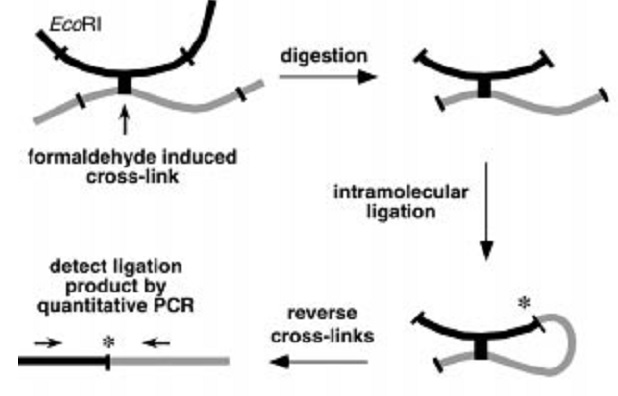
\includegraphics[scale=0.3]{3Cschematic}
\end{figure}
\end{frame}

\subsubsection{The experimental Data}\label{subsubsection_theExperimentalData}

\begin{frame}{The experimental data}
\begin{itemize}
\item Two replicate of the 5C experiments were conducted by Nora et. al 2012. 
\item Undifferentiated mouse embryonic stem cells.
\item We focus on a 920,432 bp subset of the data, around the X inactivation center of the X chromosome. 
\item The region harbors the Xist enhancer and Tisx promoter.
\item The subset of the data contains two adjacent Topologically Associating Domains (TADs).
\end{itemize}
\end{frame}

\begin{frame}{Topologically Associating Domains (TADs)}
Conserved structures showing chromosome interactions on the Mb scale, with higher intra than inter-region interactions.
It is believed that the TAD forms a 'regulatory unit' for gene expression.
However, its existence and role are not completely verified in a single cell.
\centering
\begin{figure}[H]
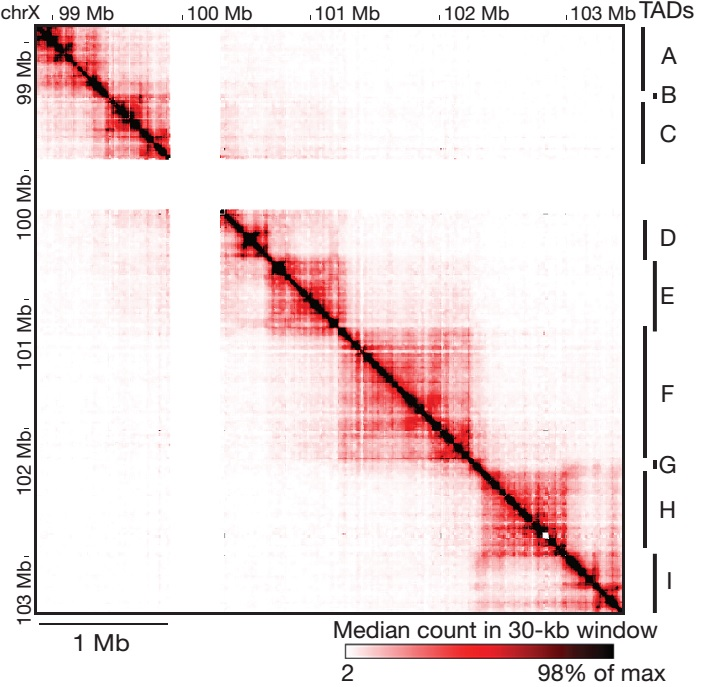
\includegraphics[scale=0.2]{TADsOfTheXChromosome_NoraEtAl2012}
\quad
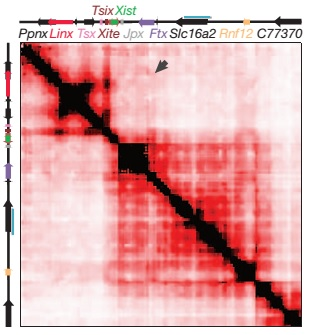
\includegraphics[scale=0.25]{TadDandENoraEtAl2012} 
\quad
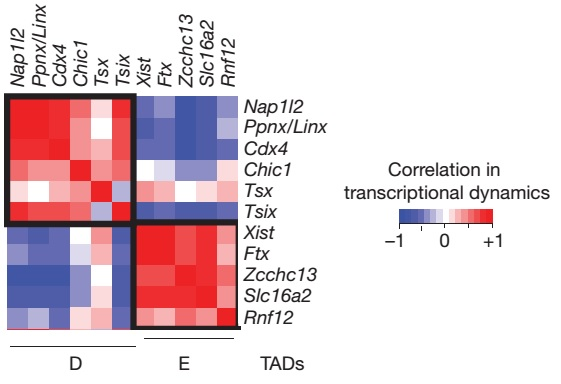
\includegraphics[scale=0.27]{transcriptionCorrelationTadDandENoraEtAl2012}
\caption{\tiny{The 4.5 Mb region (left), enlargement of TAD D and E (center). Displayed median count in a 30kb window every 6kb, gene expression Peasrsons correlation (right)}}
\label{fig:TADsOfTheXChromosome_NoraEtAl2012}
\end{figure}
\end{frame}

\subsection{Analysis of the data}\label{subsection_analysisOfTheData}

\begin{frame}{From restriction segments to beads}
\begin{itemize}
\item Coarse-graining of the data was made by choosing a bead-size of 3000 bp, corresponding to the mean segment length resulted from the digestion of HindIII. 

\begin{figure}[H]
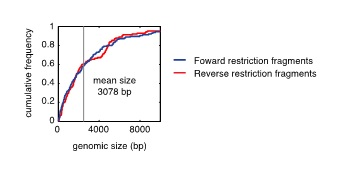
\includegraphics[scale=0.55]{restrictionSegmentLengthDistributionLucaetal}
\end{figure}
\item The genomic section was evenly partitioned. Each bead receives a start and end index according to the segment it covers. 
\item for example: 
\begin{tabular}[H]{|l| l| l|}
\hline
bp range & start ind & end ind\\
\hline
500-3500   & 1         & 2 \\
4000-4500  & 2         & 2 \\   
5000-12001 & 2         & 4 \\       
\hline  
\end{tabular}
\end{itemize}
\end{frame}

\subsubsection{TAD D and E}\label{subsubsection_tadDAndE}

\begin{frame}{Bead encounter probability}
\framesubtitle{TAD D and E}
\begin{itemize}
\item We work with the average of the two experimental replicates.
\item A total length of 920,432 bp - resulting in 307 beads (TAD D 107 beads, TAD E 200 beads).
\item For each bead we calculate the encounter probability as a function of distance (bead units).
\item TAD E has several strong specific interactions. TAD D has weak intra long range interactions. Strong inter-TAD specific interactions
\end{itemize}

\begin{figure}[H]\label{TADDAndEencounterProb}
\centering
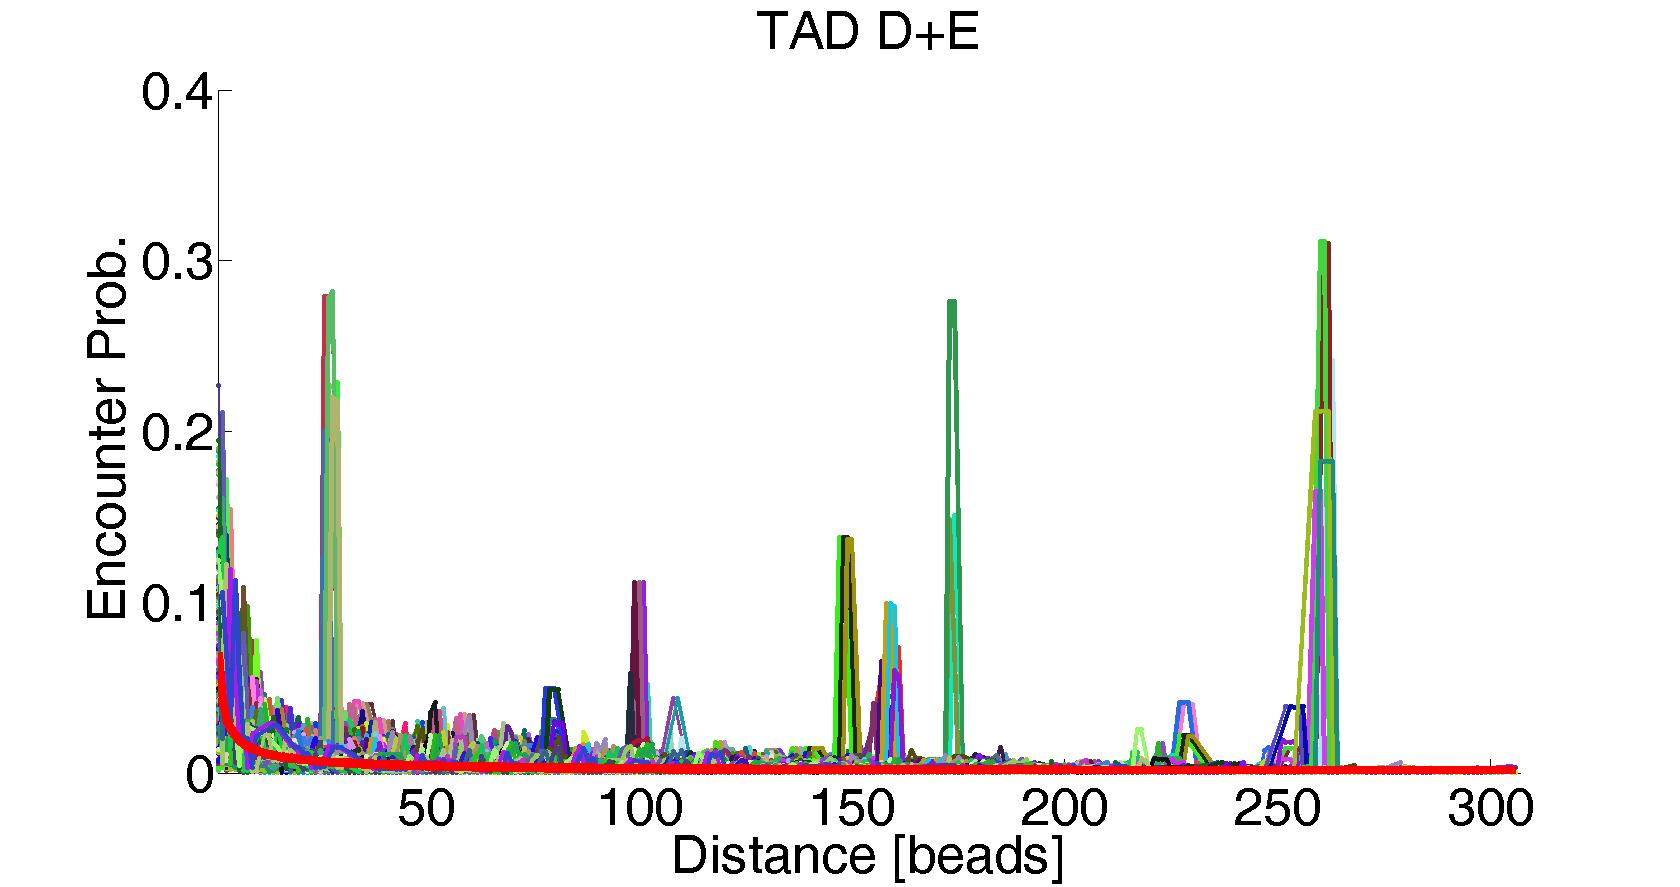
\includegraphics[scale=0.078]{encounterProbabilityTADDAndE}
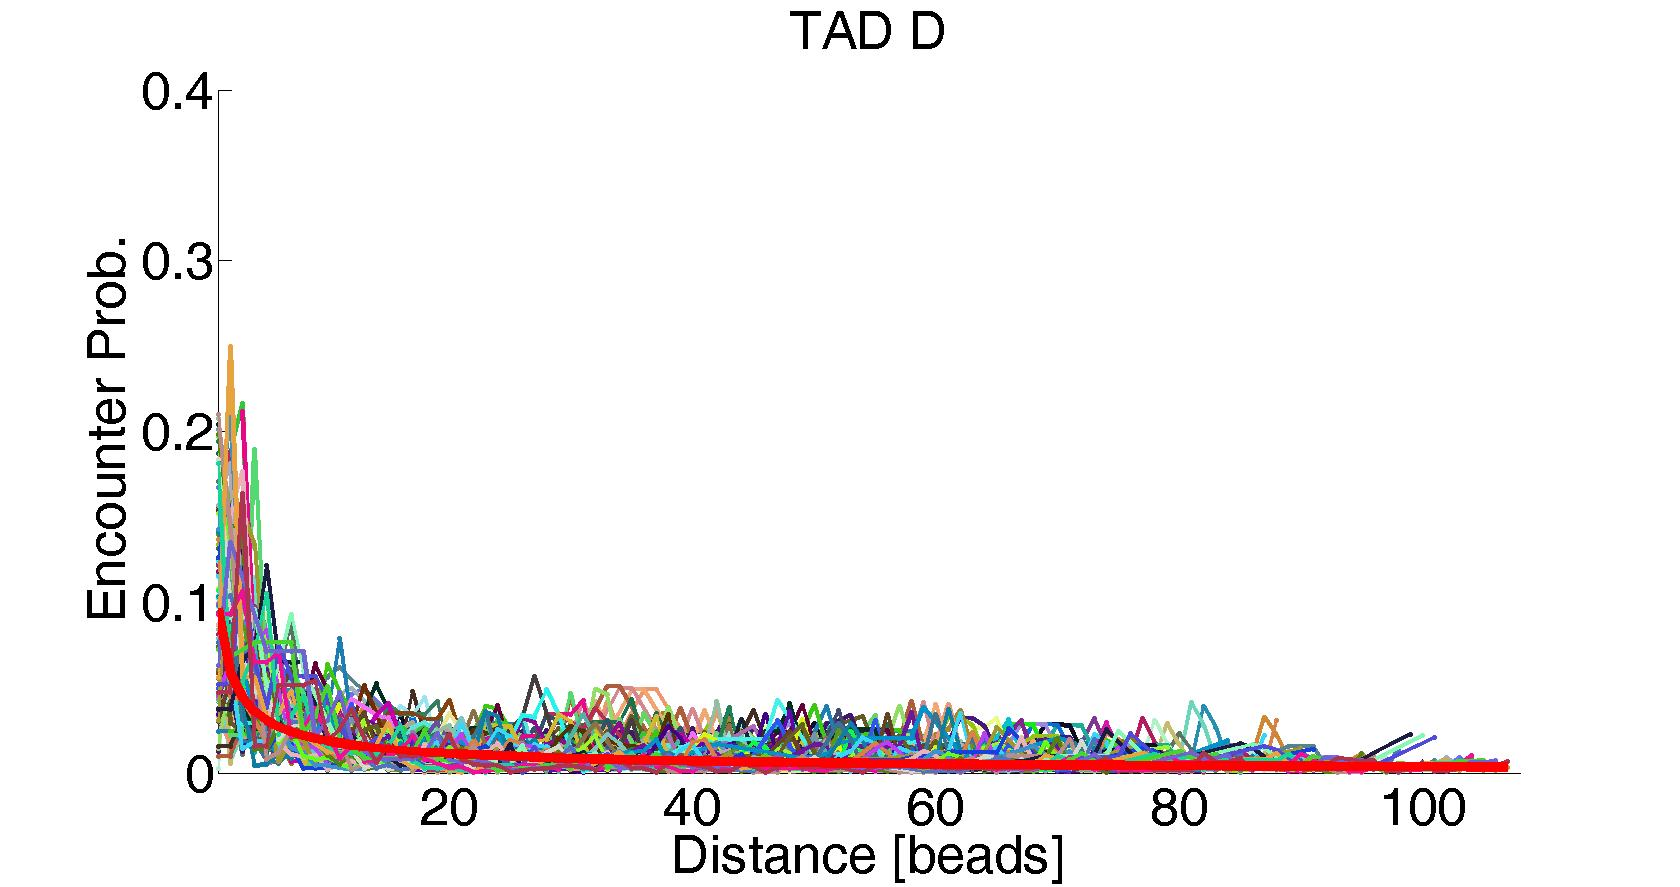
\includegraphics[scale=0.075]{encounterProbabilityTADD}
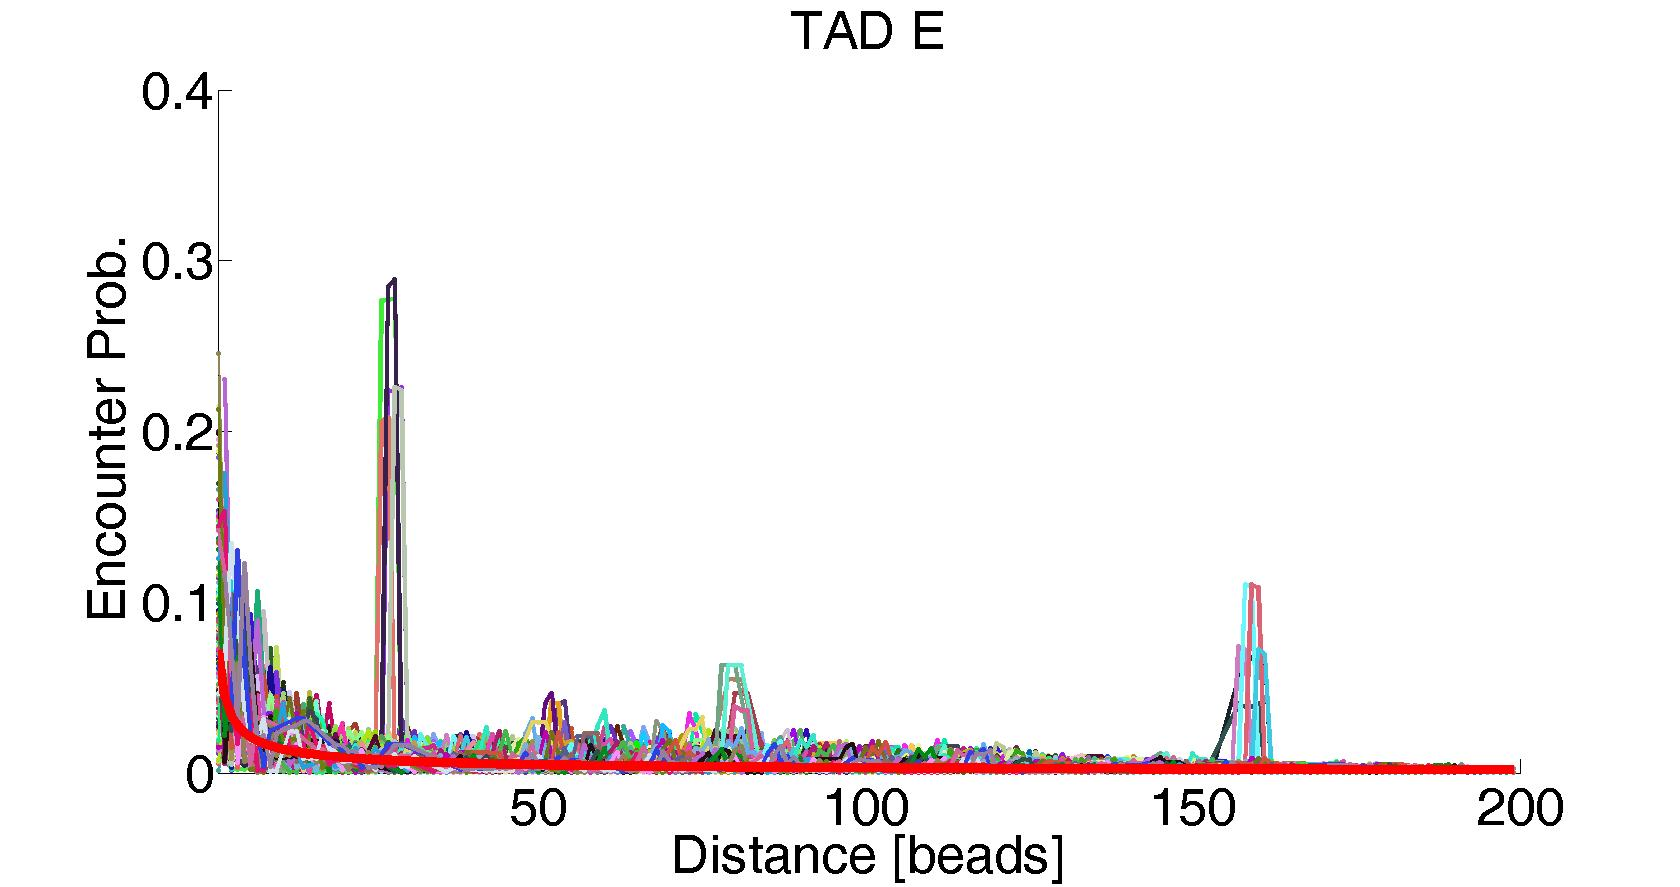
\includegraphics[scale=0.075]{encounterProbabilityTADE}
\end{figure}
\end{frame}

\subsection{Theoretical model}\label{section_theoreticalModel}

\begin{frame}{Theoretical model}
\framesubtitle{The Rouse model}
To understand the dynamical process underlying the observed encounter probabilities we need a employ a polymer model. We start with the classical and most simple model, the Rouse chain.
\begin{itemize}
\item A Rouse chain describes polymer dynamics as a stochastic motion of a collection of microscopic "beads" connected by harmonic springs
\item the 3D  motion of bead $n$ in the chain of $N$ beads 
\begin{equation*}
\frac{dR_n}{dt} = -\frac{3D}{b^2}(2R_n(t)-R_{n+1}(t)-R_{n-1}(t))+f_n(t)
\end{equation*}
\item $R_n$- the position of bead $n$\\
$b$- the standard deviation of the distance between adjacent beads\\
$D$- the diffusion constant\\
$f_n$- white Gaussian noise
\item From the theory, $Pr(\|R_n-R_m\|<\epsilon)\sim  |n-m|^{-1.5}$
\end{itemize}

\begin{figure}[H]
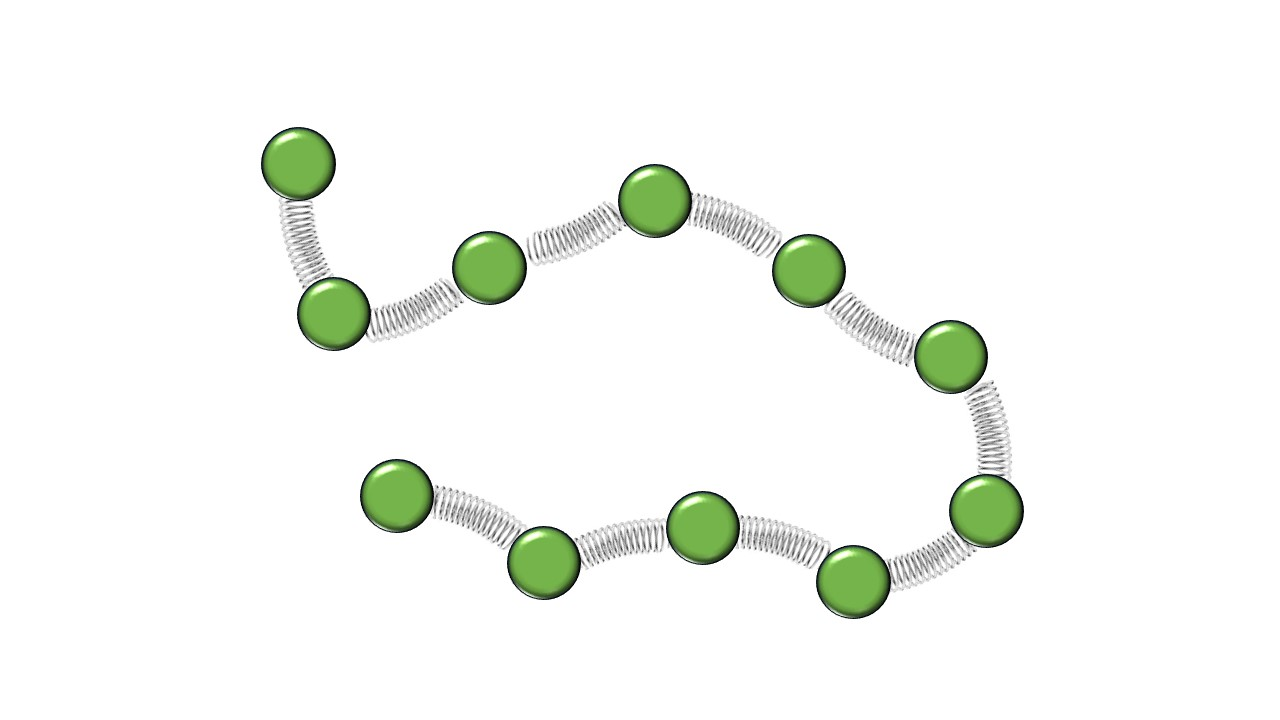
\includegraphics[scale=0.1]{RousePolymerSketch}
\end{figure}
\end{frame}

\subsubsection{The encounter probability}\label{subsubsection_theEncounterProbability}

\begin{frame}{The enconter probability}
For the case of TAD D, TAD E, and the two together, we estimate the bead encounter probability, $p$, and fit it with a function of the form 
\begin{equation*}
p_n(d)=\alpha d^{-\beta}
\end{equation*}
where, $d$ is the distance in [bead] units, $n$ is the bead number, $\alpha=\frac{1}{\sum_{j=1}^{d_{max}}j^{-\beta}}$ and $\beta$ is a parameter to be estimated.
We report the values of $\beta$ for each bead in each case.
\begin{figure}[H]
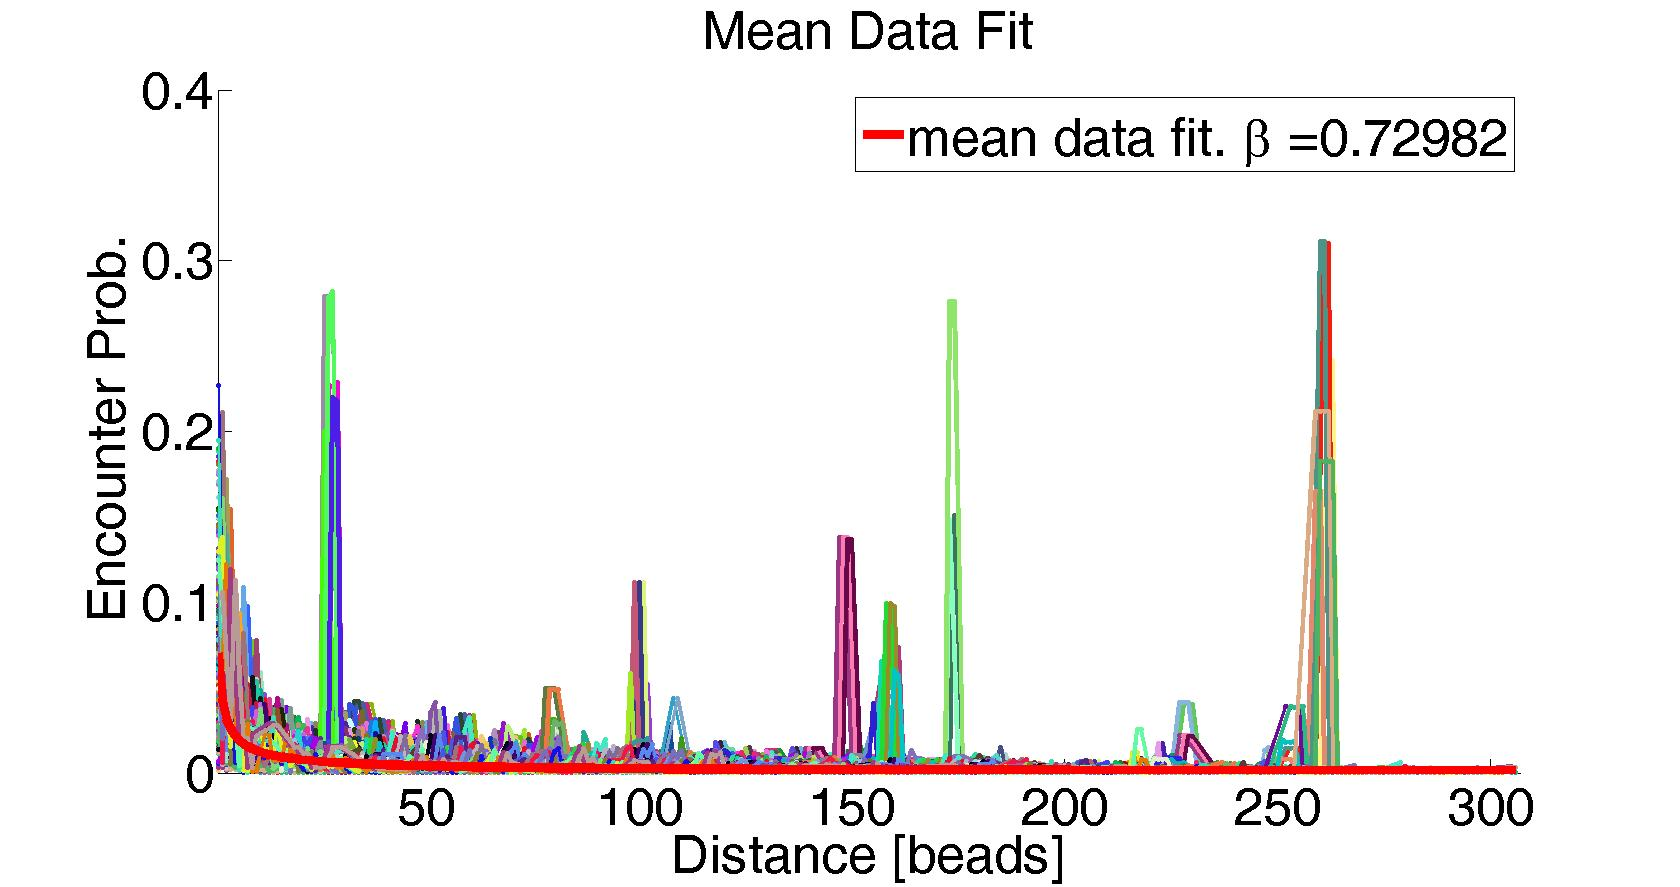
\includegraphics[scale=0.1]{meanDataFitTADDAndE}
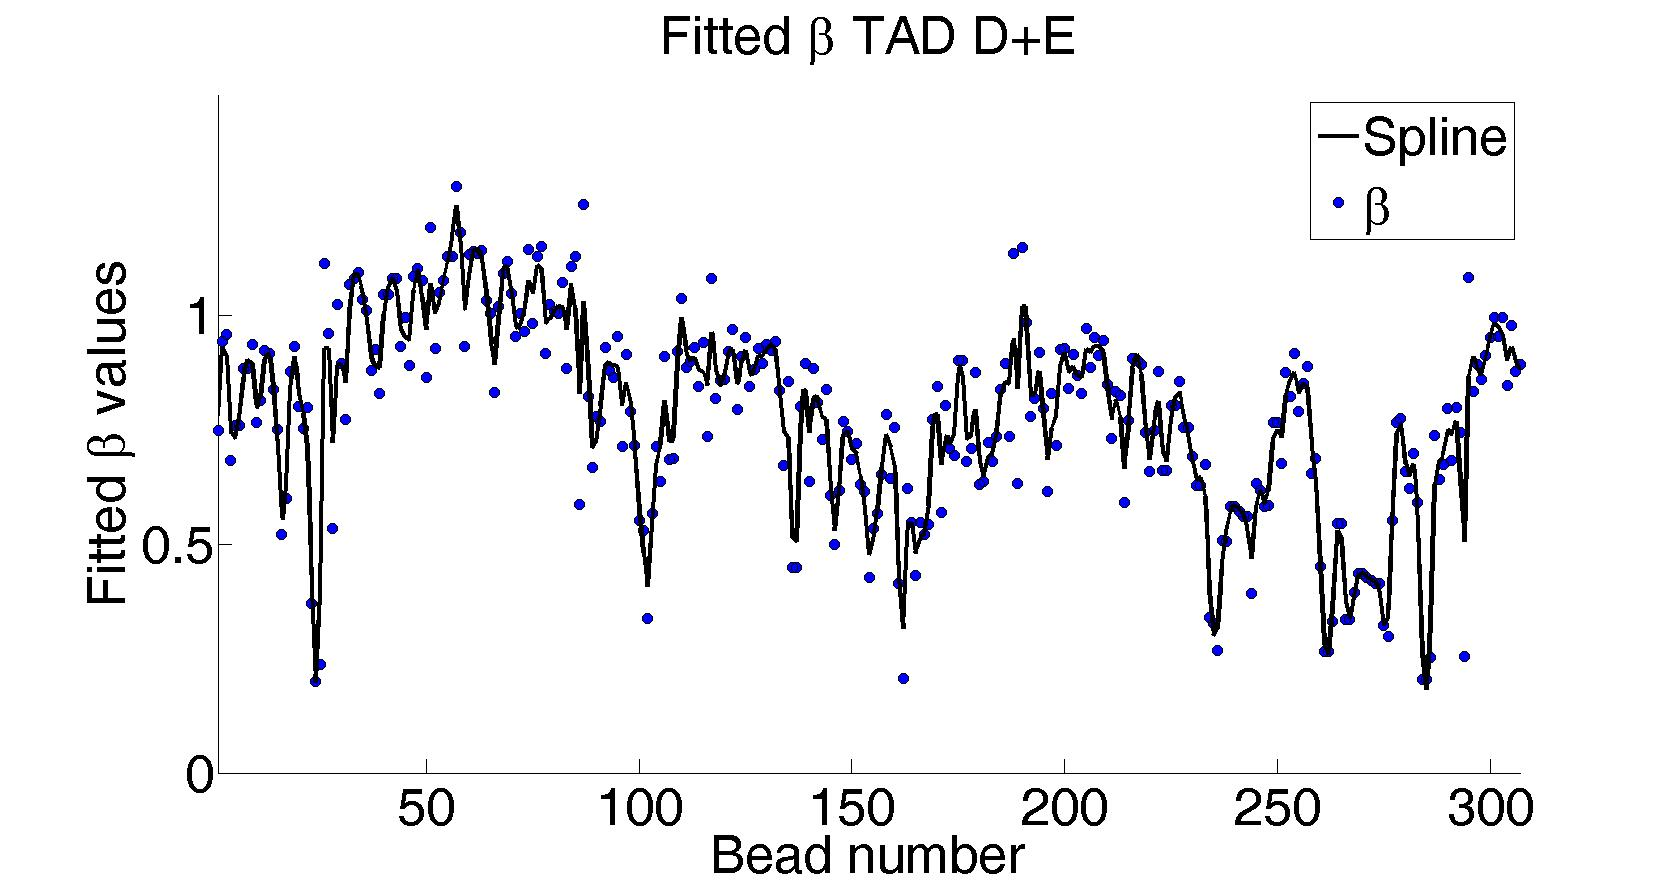
\includegraphics[scale=0.1]{fittedExpValuesWithSplineAverageTADDAndE}
\end{figure}
\end{frame}

\begin{frame}
\framesubtitle{TAD D and E}
\begin{figure}[H]
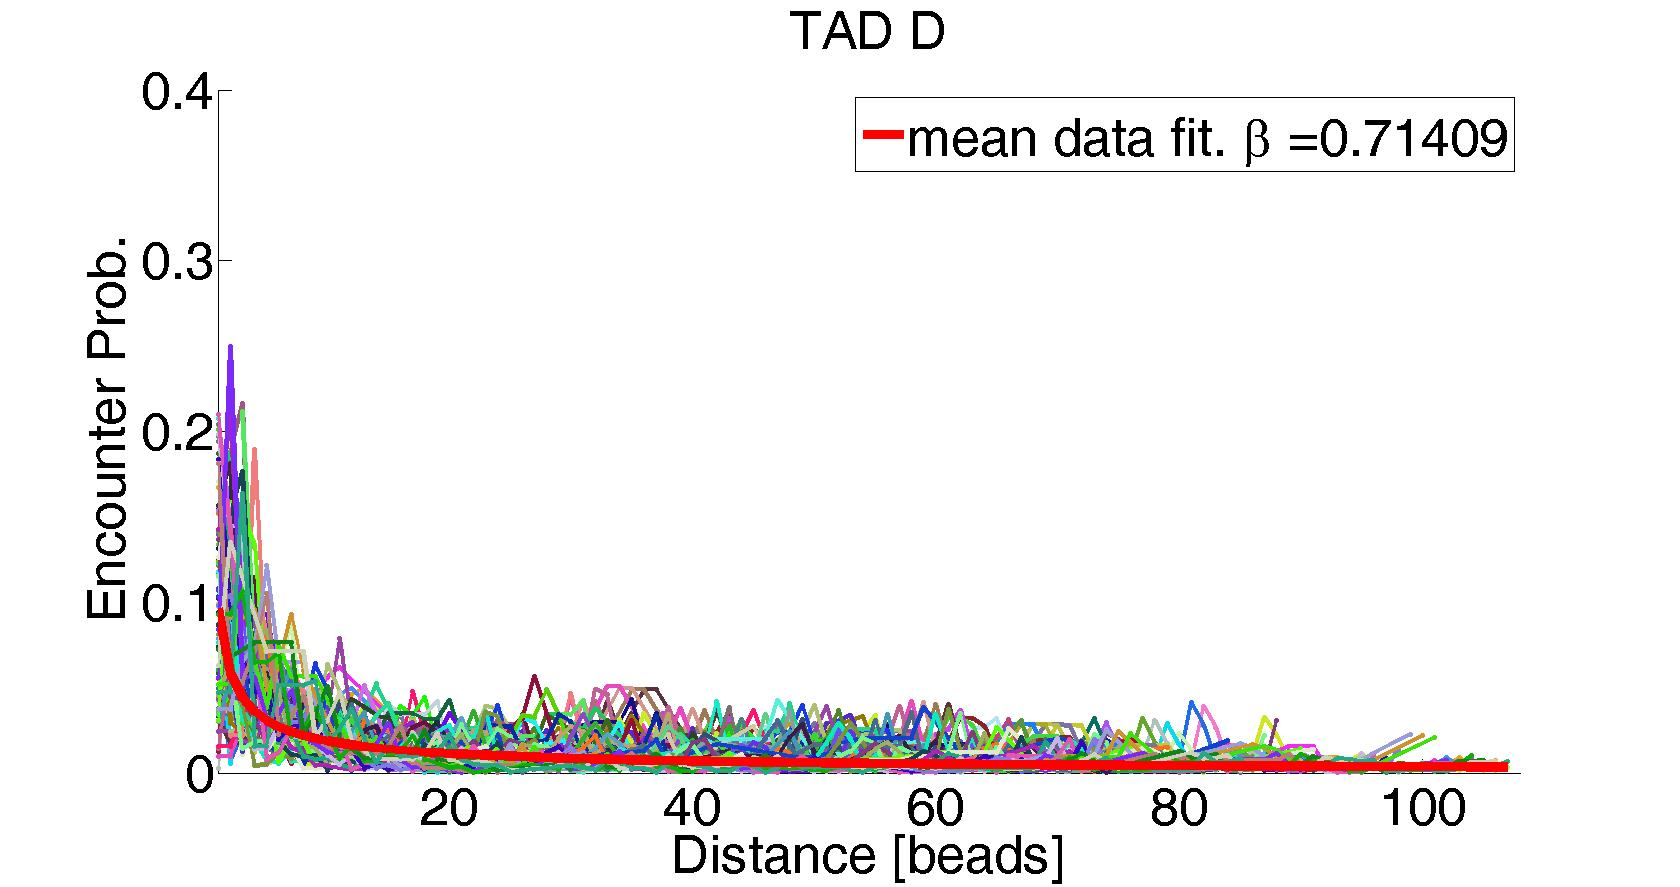
\includegraphics[scale=0.1]{meanDataFitTADD}
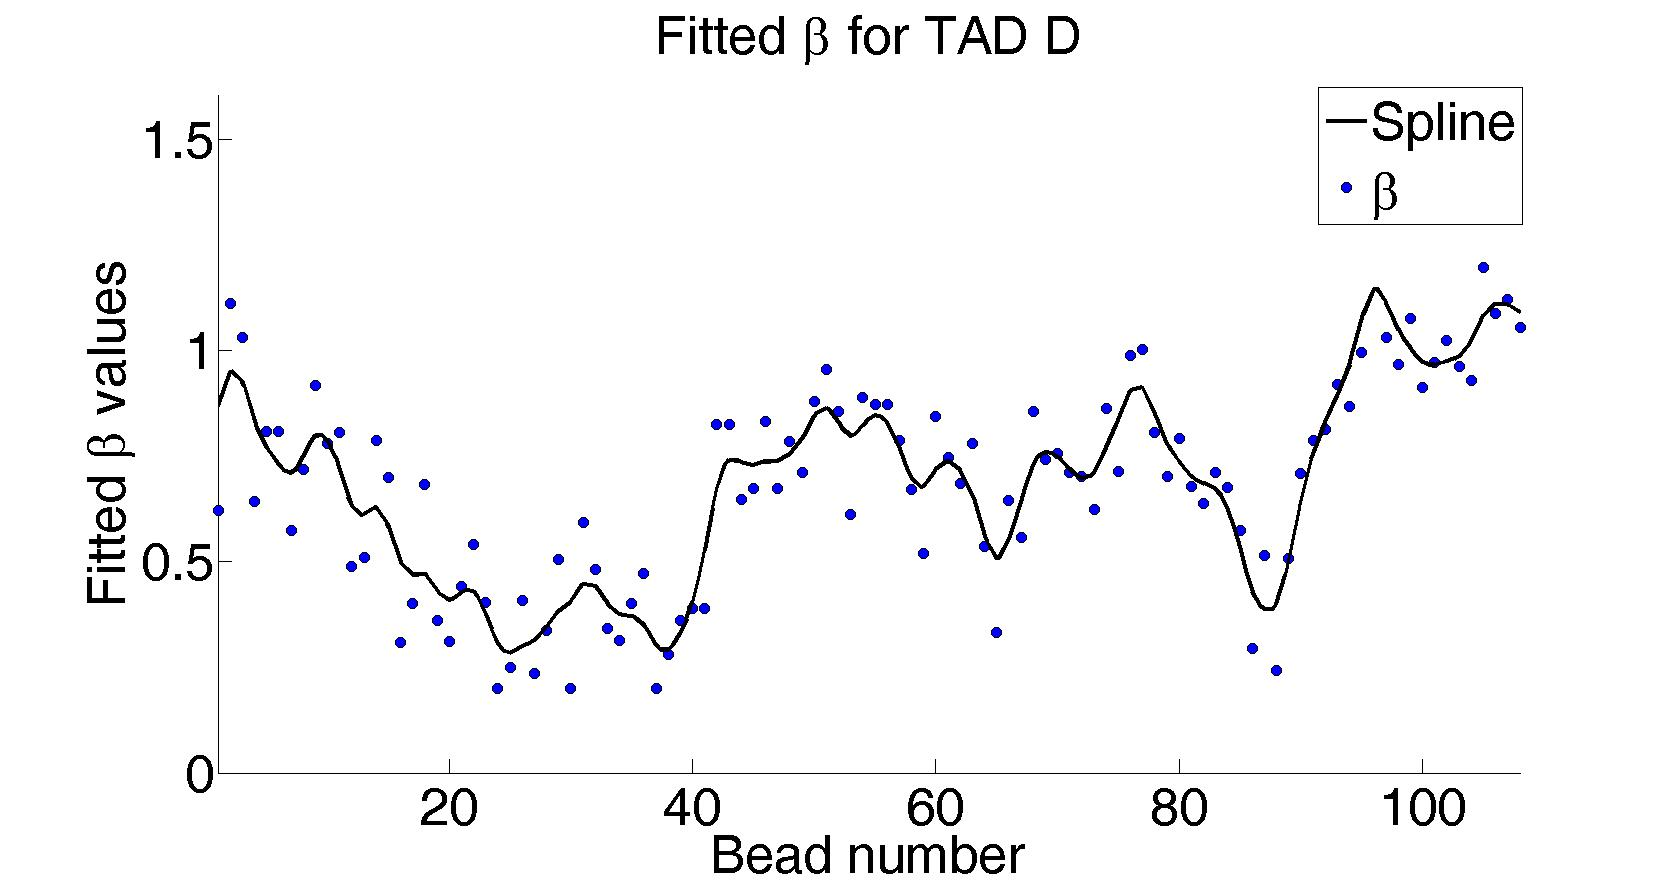
\includegraphics[scale=0.1]{fittedExpValuesWithSplineAverageTADD}
\end{figure}

\begin{figure}[H]
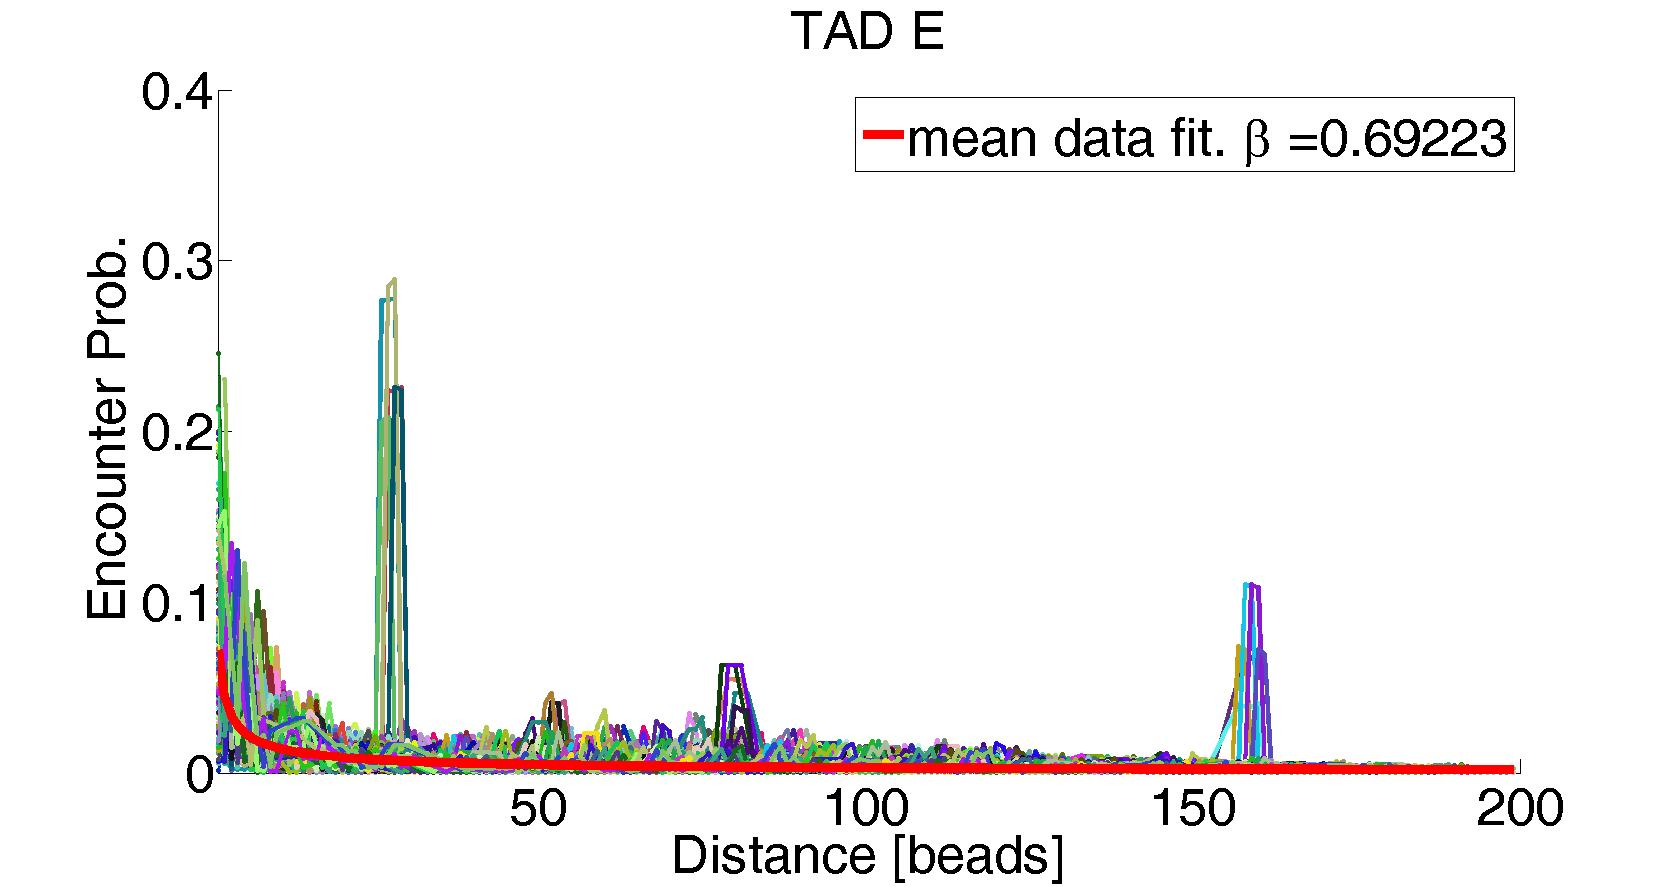
\includegraphics[scale=0.1]{meanDataFitTADE}
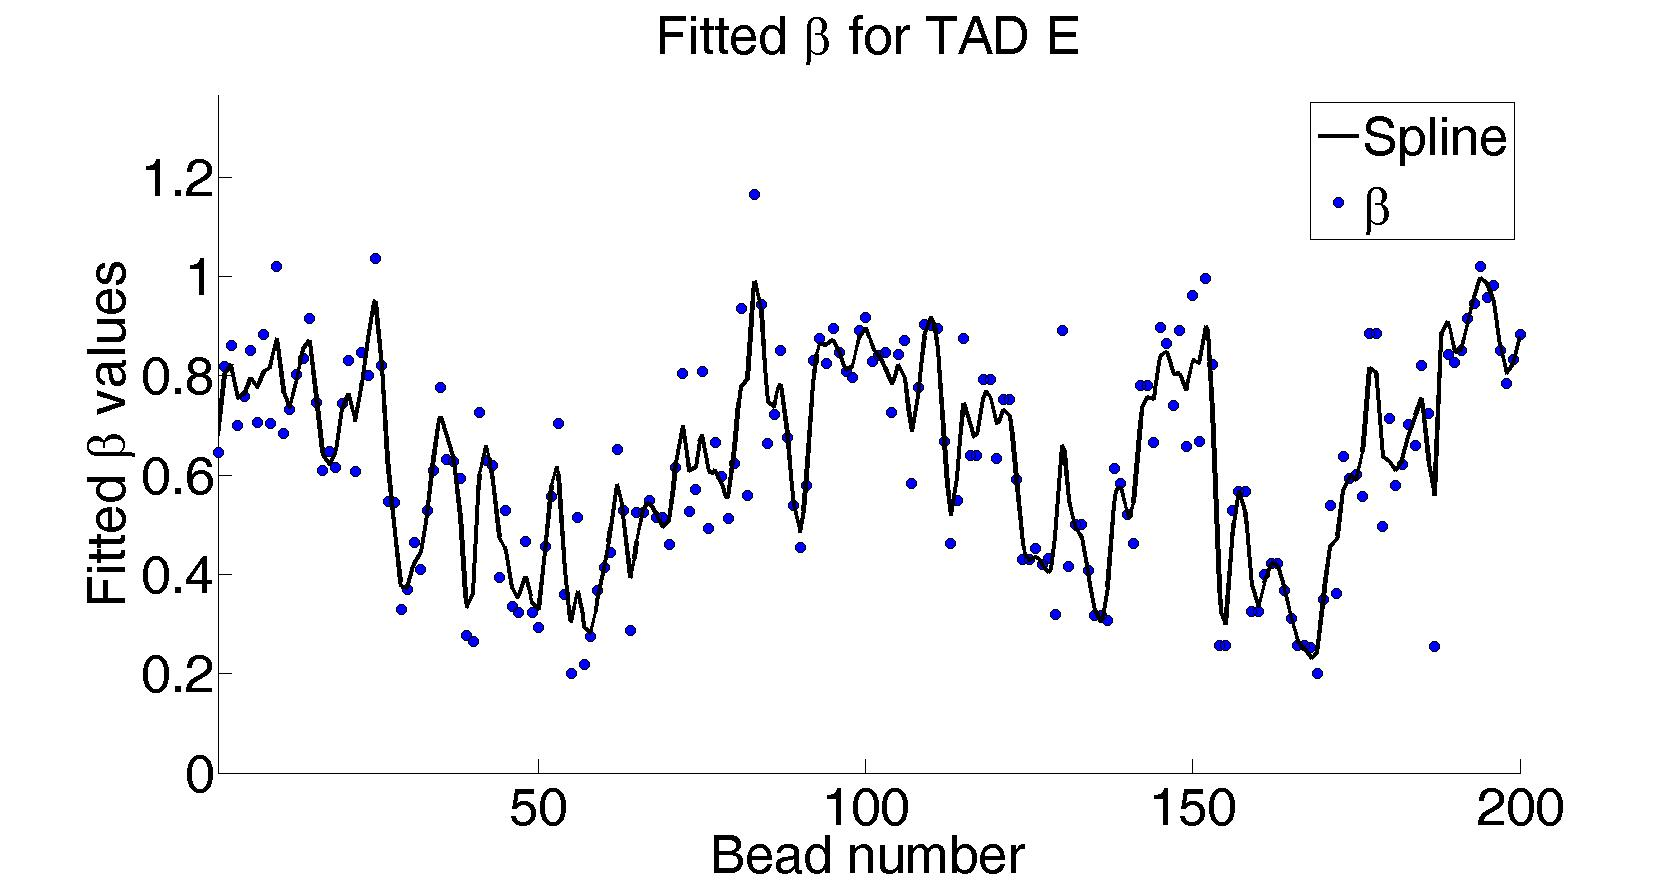
\includegraphics[scale=0.1]{fittedExpValuesWithSplineAverageTADE}
\end{figure}
\end{frame}

\subsubsection{Peaks of the encounter data}\label{subsubsection_peaksOfTheEncounterData}

\begin{frame}{Peaks of the encounter data}
\begin{itemize}
\item A peak-calling procedure was implemented to find pairs of beads which interact frequently. 
\item Peak analysis was performed separately for TAD D, E and between TADs. 
\item About $90\%$ of the peaks in the encounter data result from specific interactions between TADs and in TAD E.
\end{itemize}
\begin{figure}[H]
\includegraphics[scale=0.15]{peakListAverage}
\end{figure}

\end{frame}

\subsection{Simulation Results}\label{subsection_simulationResults}
%simulation section order:
% 1. normal Rouse 
% 2. normal rouse with peaks
% 3. rouse with random loops one TAD with tails 
% 4. rouse with random fixed loops in two TADs

\subsubsection{Simulations with a simple rouse chain}\label{subsubsection_simulationWithSimpleRouse}

\begin{frame}{Simulation with simple rouse chain}
\begin{itemize}
\item A simple Rouse model cannot reproduce the TAD, as expected.
\item Placing loops corresponding to the peaks of the encounter data does not reproduce the TADs. 
\end{itemize}
\begin{figure}[H]
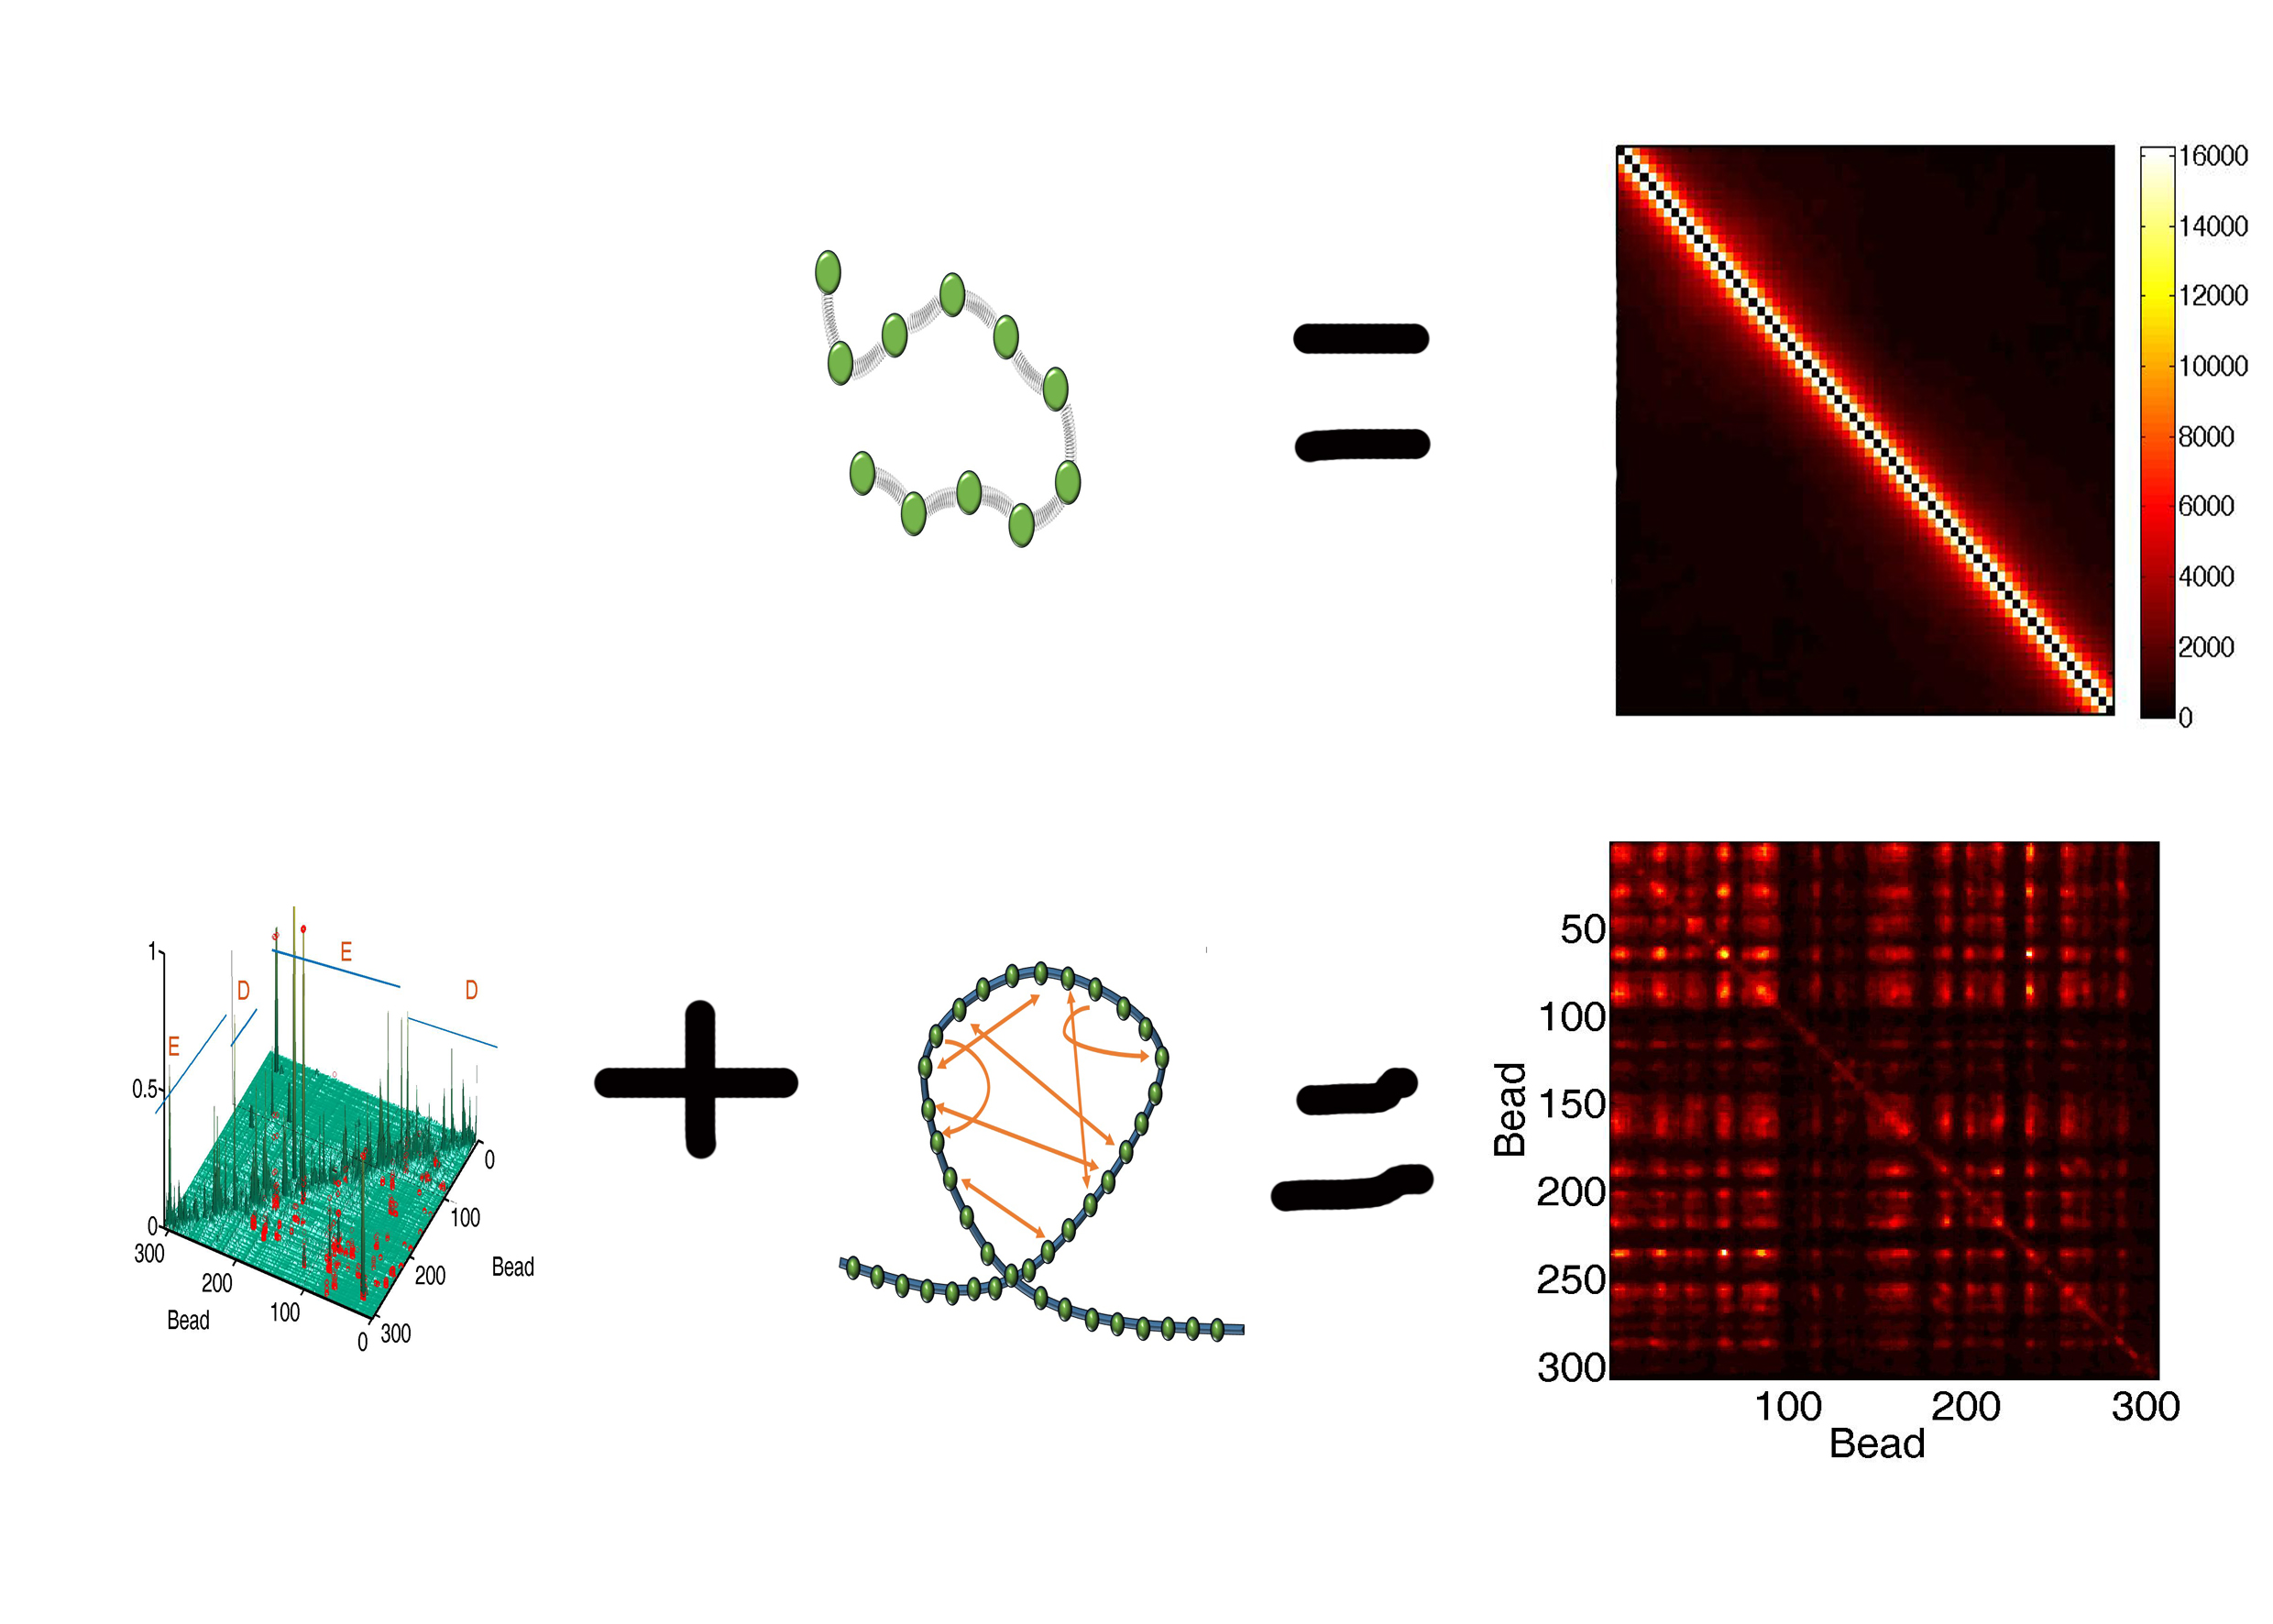
\includegraphics[scale=0.4]{simulationWithSimpleRouseExperimentalData}
\end{figure}
\end{frame}

\subsubsection{Random loops model}\label{subsubsection_randomLoopsModel}

\begin{frame}{Random Fixed Loop Model}
\begin{itemize}
\item The enhancer-transcription factor elements' encounter motivates the simulation of a chain with randomly placed loops.
\item These encounters might not be as frequent as 'stable' loops in the chromatin and therefore not shown significantly in the encounter maps.
\item Simulate a chain of 307 beads, having random loops in a bounded region.
\item Increasing number of loops at random positions. 
\end{itemize}

\end{frame}

\begin{frame}{Stable loop with random loops within}
\framesubtitle{one TAD}
\begin{enumerate}
\item Following the peaks observation, we form a mix of 'stable' big loop with internal random loops.
\item In a 307 beads chain, beads 107 and 207 were connected.
\item We iteratively add up to 30 connectors within the stable big loop.
\item We can start seeing the emergence of $\beta$ curve pattern as in the experimental data.
\end{enumerate}
\begin{figure}[H]
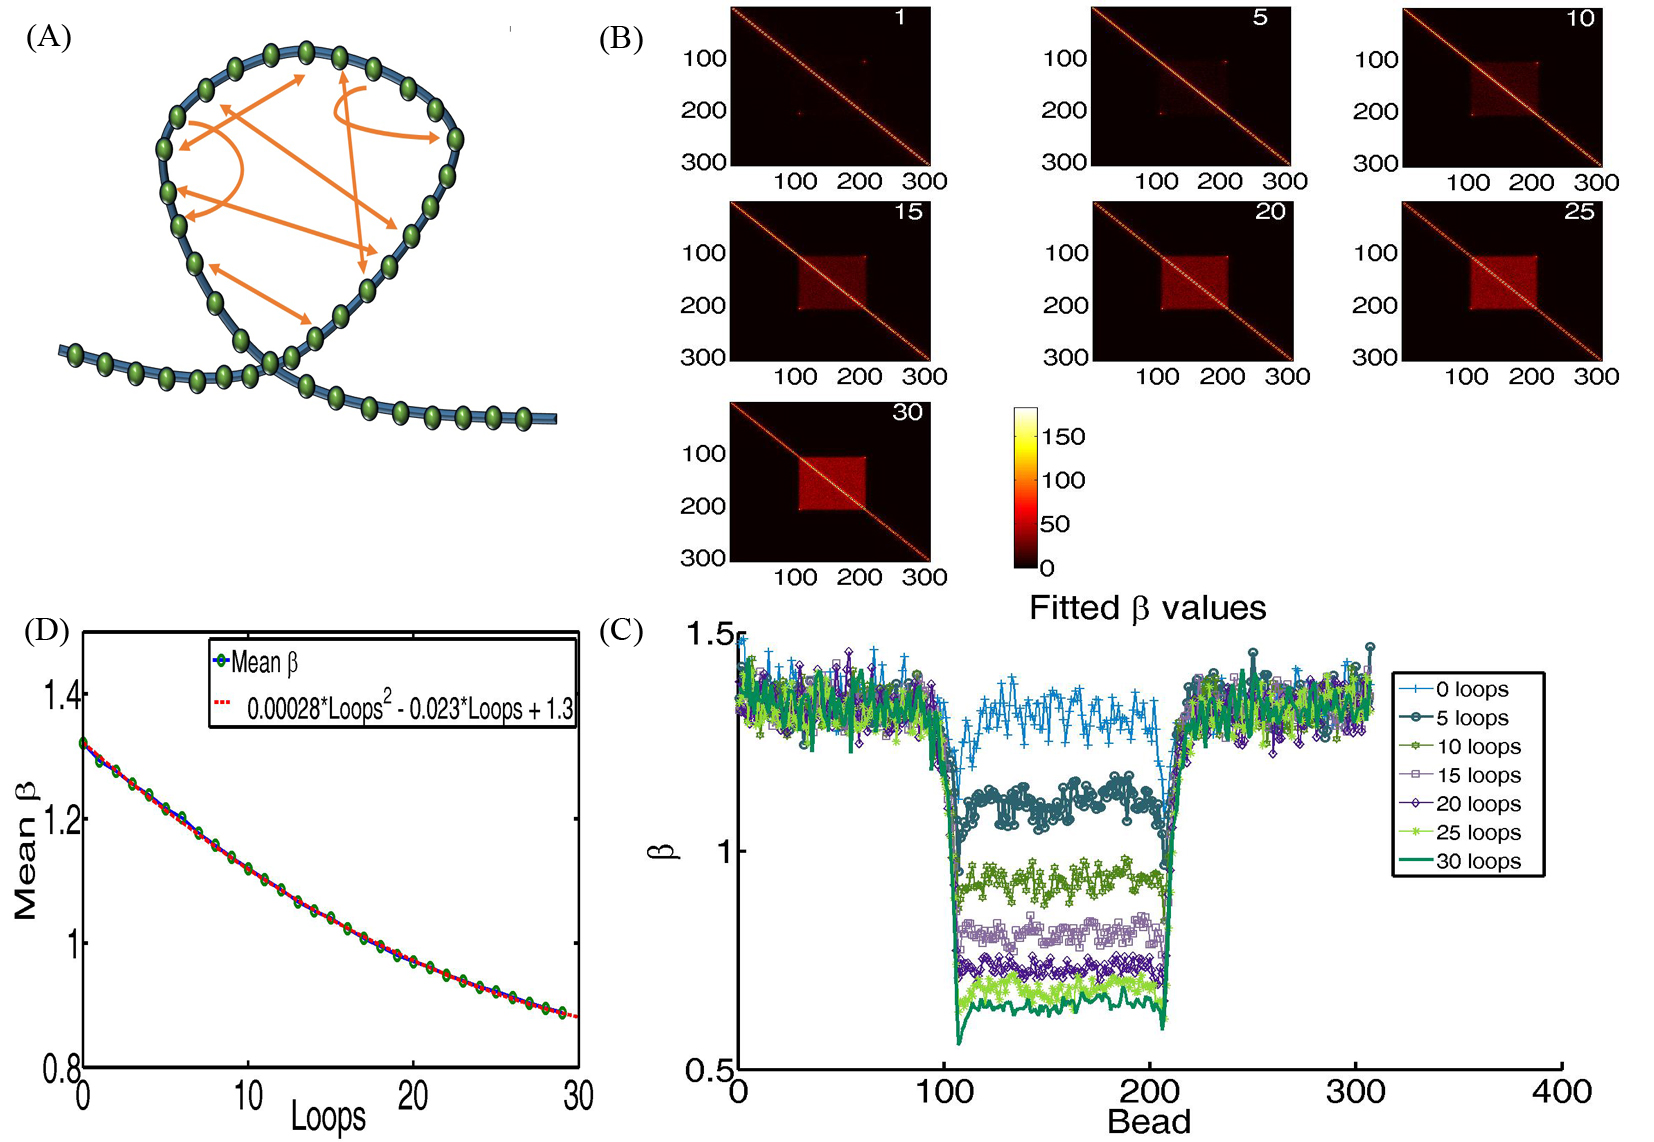
\includegraphics[scale=0.35]{Figure03_OneTADWithTails0To30RandomLoops}
\end{figure}
\end{frame}


\begin{frame}{Stable loop with random loops within}
\framesubtitle{Two TADs}
\begin{enumerate}
\item In a 307 beads chain, we create two stable loops by connecting bead 1 and 107, and bead 108 and 307
\item We iteratively add 30 connectors within each TAD.
\item We can start seeing the emergence of $\beta$ curve pattern as in the experimental data.
\end{enumerate}
\begin{figure}[H]
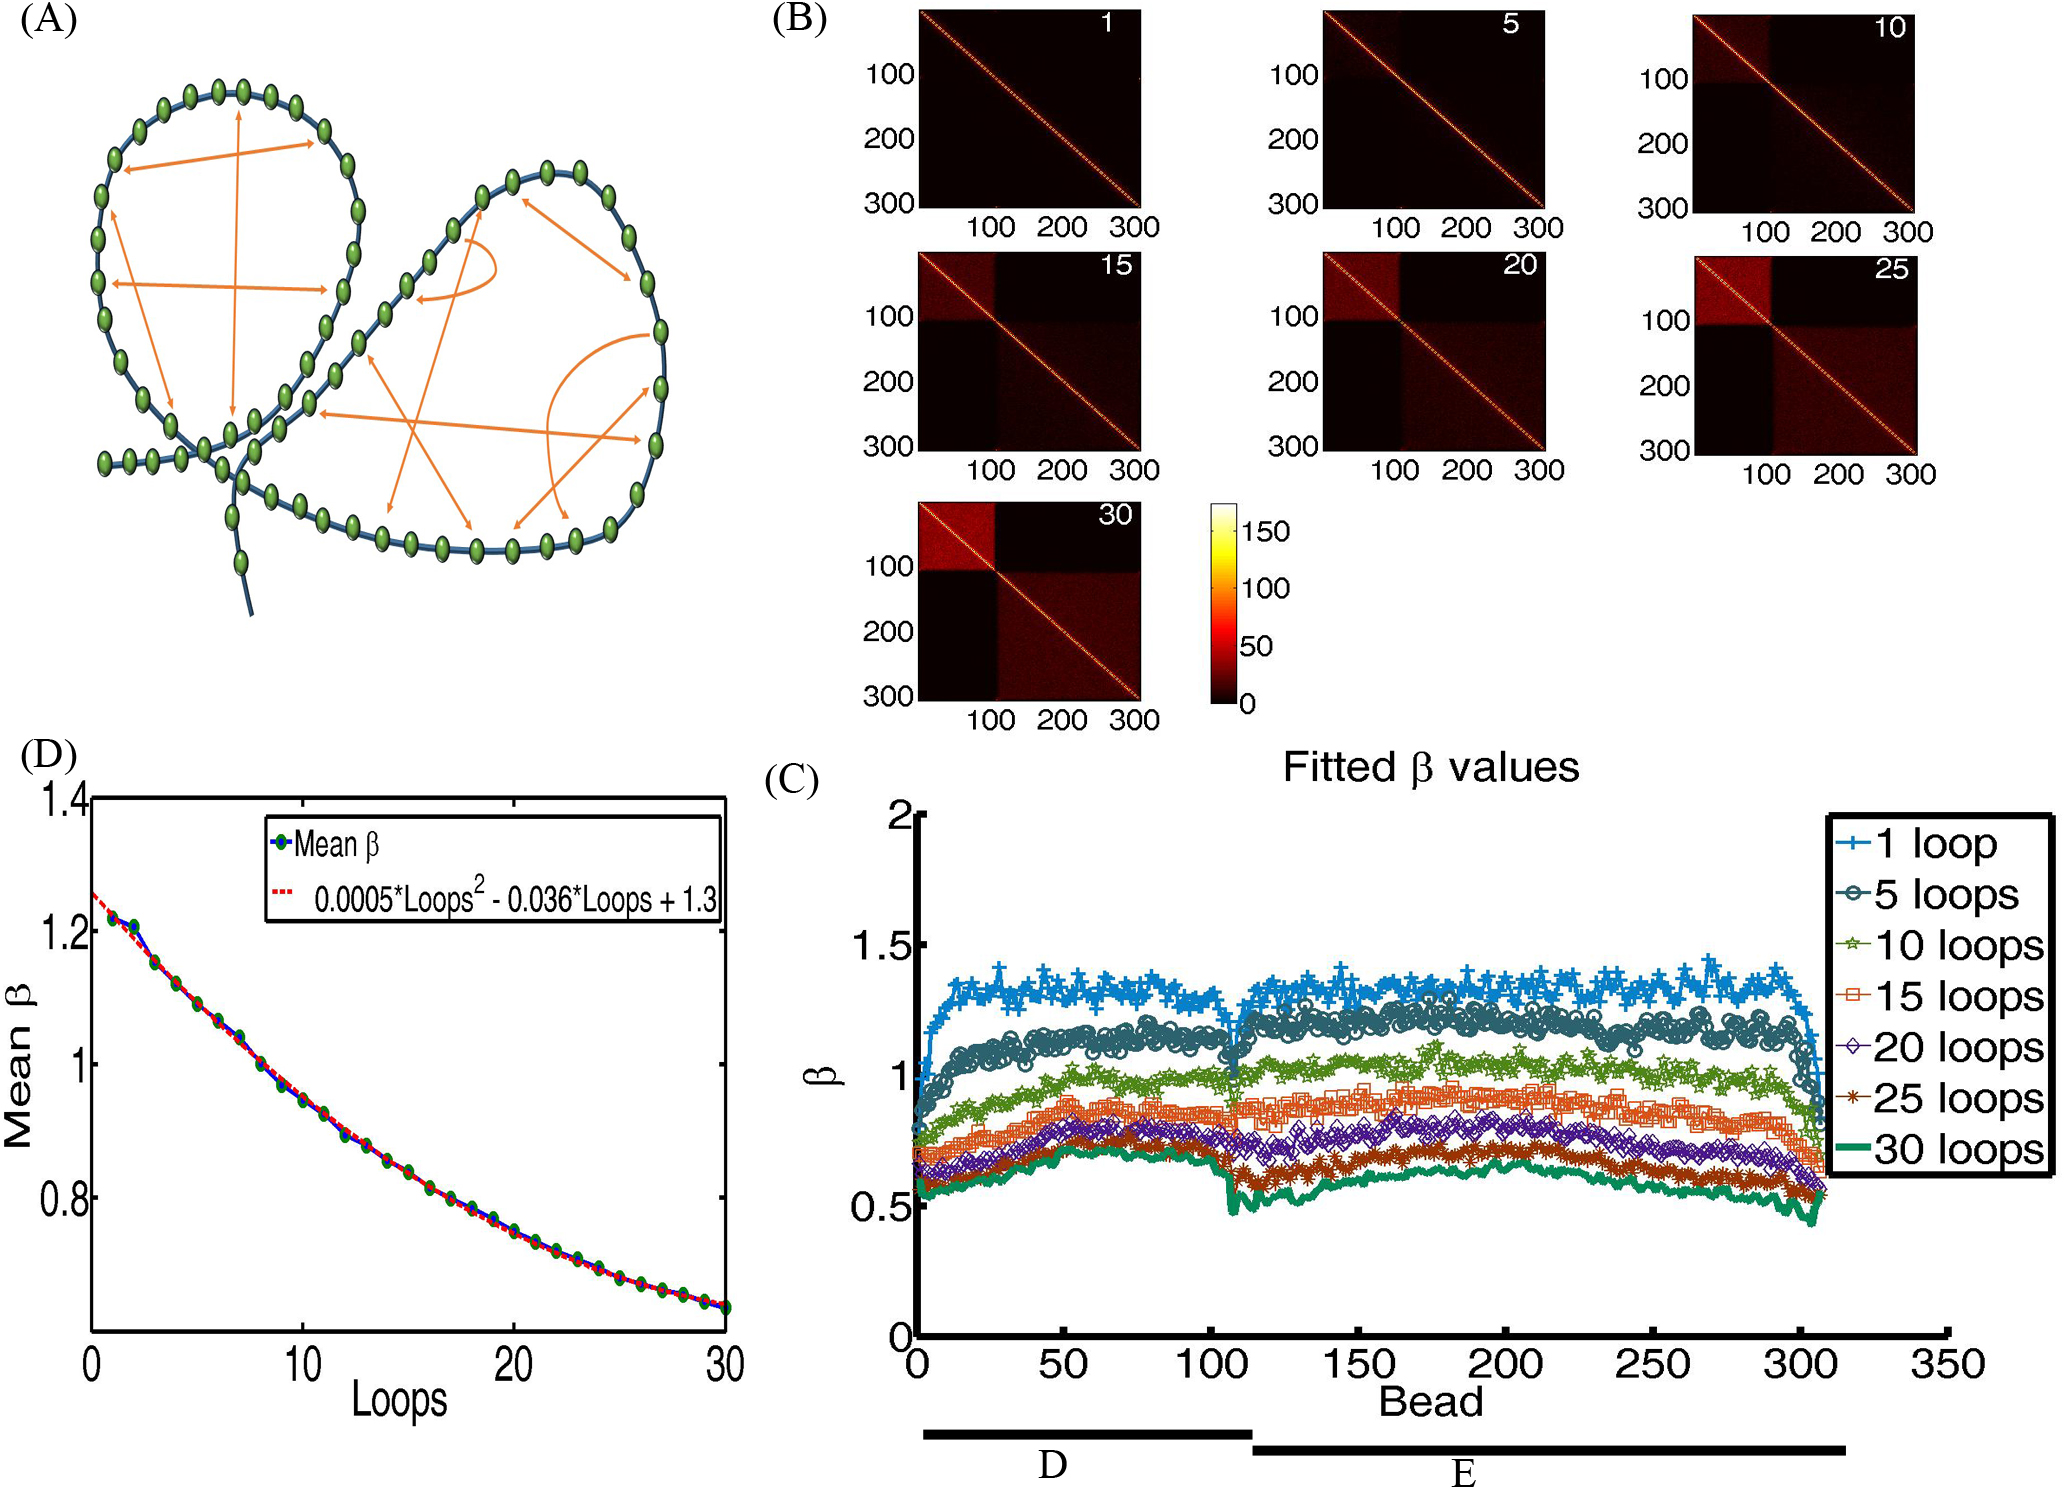
\includegraphics[scale=0.35]{Figure04_TwoTADs0To30RandomLoops307Beads}
\end{figure}
\end{frame}


\subsection{Summary}\label{subsection_summaryAndFutureWork}

\begin{frame}{Summary}
\begin{itemize}
\item We presented a plausible and simple model to explain the appearance of the conserved TAD domains. 
\item The model represent the results obtained in the population level.
\item A relationship between the mean number of loops and the encounter probability was shown by simulations.
\item The parameter $\beta$ used for our analysis can easily be retrieved from the experimental data. 
\end{itemize}
\end{frame}

\begin{frame}{Work in progress}
\begin{enumerate}
\item Calculating the conditional probability of bead A meeting bead B before it mets bead C in the resulting polymer configuration. 
\item Calculation of the mean first encounter time between beads in random loop model 
\item Showing analytically the relationship between number of loops and decrease in $\beta$
\item Put in more rigorous form the relationship between the pattern of $\beta$ and the mean observed chromatin structure.
\item constructing a heterogeneous random loop model, taking into account the peaks and varying spring constants.
\item Simulating a model with random dynamic loops, in which loops can form and dissociate.
\item simulating the beta polymer with random loops. 
\item Experiment with other polymer models.
\end{enumerate}
\end{frame}

\section{Part II - Reconstruction}\label{section_partII} 
\begin{frame}{Part II Reconstruction}
\begin{enumerate}
\item How do we go from encounter frequencies to structure?
\item Allow us to studying prominent features of the structure 
\item Allow us to perform non-equilibrium simulations in complex structures inferred from experimental data. 
\item The encounter data holds a lot of spatial information 
\item We will show a method to exploit the encounter probabilities to infer a structure
\end{enumerate}
\end{frame}

\subsection{The theoretical model}\label{subsubsection_theRouseEncounterProbability}
\begin{frame}{The encounter probability in the Rouse chain}
We begin by employing a Rouse chain of $N_c$ beads to represent the chromatin.

The pdf of a vector, $R_{mn}$ between bead $m$ and $n$ in equilibrium is normal
\begin{equation*}
P(R_{mn})=\left(\frac{3}{2\pi b^2 |m-n|}\right)^{3/2}\exp\left(-\frac{3R_{mn}R_{mn}^T}{2b^2|m-n|}\right)
\end{equation*}
Setting $R_{mn}=\vec{0}$ we get the encounter probability 
$\left(\frac{3}{2\pi b^2 |m-n|}\right)^{3/2}$. 

To match the HiC signals, we normalize by dividing by 
\begin{equation*}
\sum_{t=1}^{N_C-1}\left(\frac{3}{2\pi b^2 |N-t|}\right)^{3/2}
\end{equation*}
Therefore, the encounter probability does not depend on $b^2$ 
\begin{equation*}
P(R_{mn}=\vec{0})=\frac{|m-n|^{-3/2}}{\sum_{j=1}^{N} |N_r-j|^{-3/2}}
\end{equation*}

\begin{figure}[H]
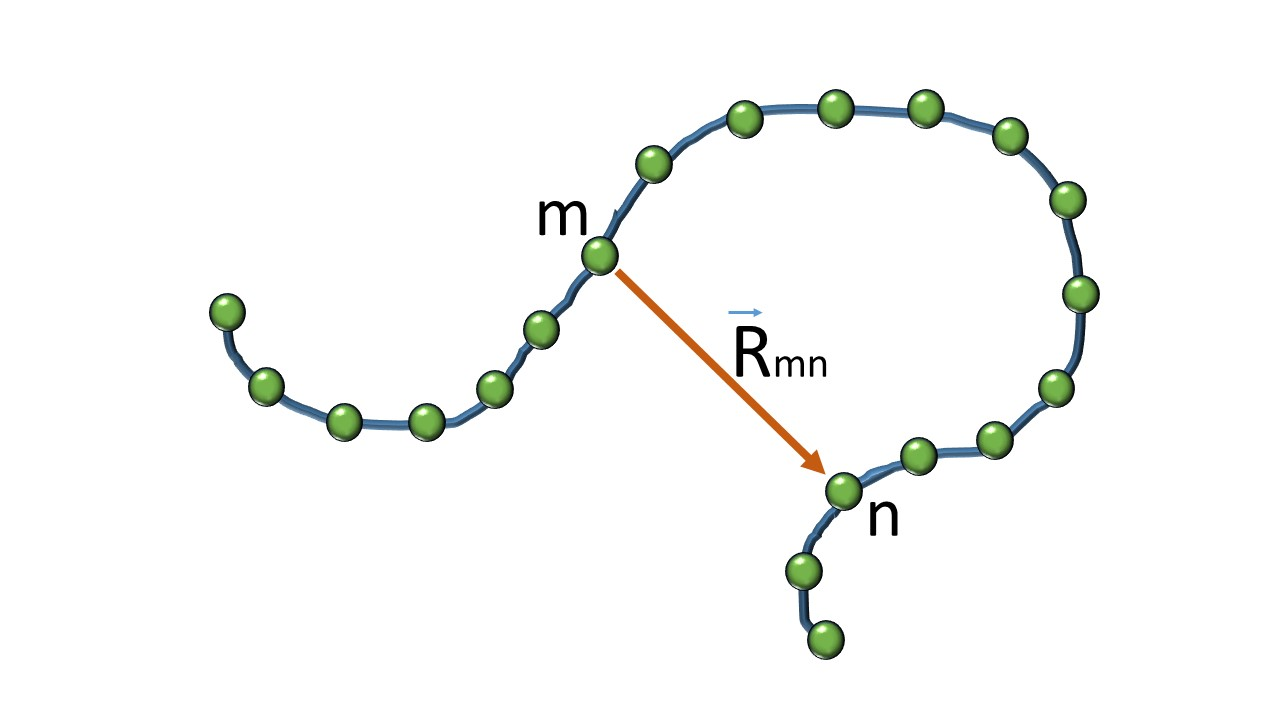
\includegraphics[scale=0.12]{rouseChainVectorBetweenMAndN}
\end{figure}
\end{frame}

\begin{frame}{The encounter probability in a ring}
Forcing the two ends of a Rouse chain to meet creates a "Rouse ring". 
A rouse ring can be represented by a Brownian bridge.
The pdf of a vector $r_{m}$ of the ring of $N_r$ beads is given by 
\begin{equation*}
P(r_m)=\left(\frac{3N}{2\pi b^2 m(N_r-m)} \right)^{3/2}\exp\left(-\frac{3N_rr_mr_m^T}{2b^2m(N_r-m)}\right)
\end{equation*}

Setting $r_m=\vec{0}$ and normalizing, we get 
\begin{equation*}
P(r_m=\vec{0})=\frac{(m(N_r-m))^{-3/2}}{\sum_{t=1}^{N_r-1}(t(N_r-t))^{-3/2}}
\end{equation*}
which also does not depend on $b^2$ 
\begin{figure}[H]
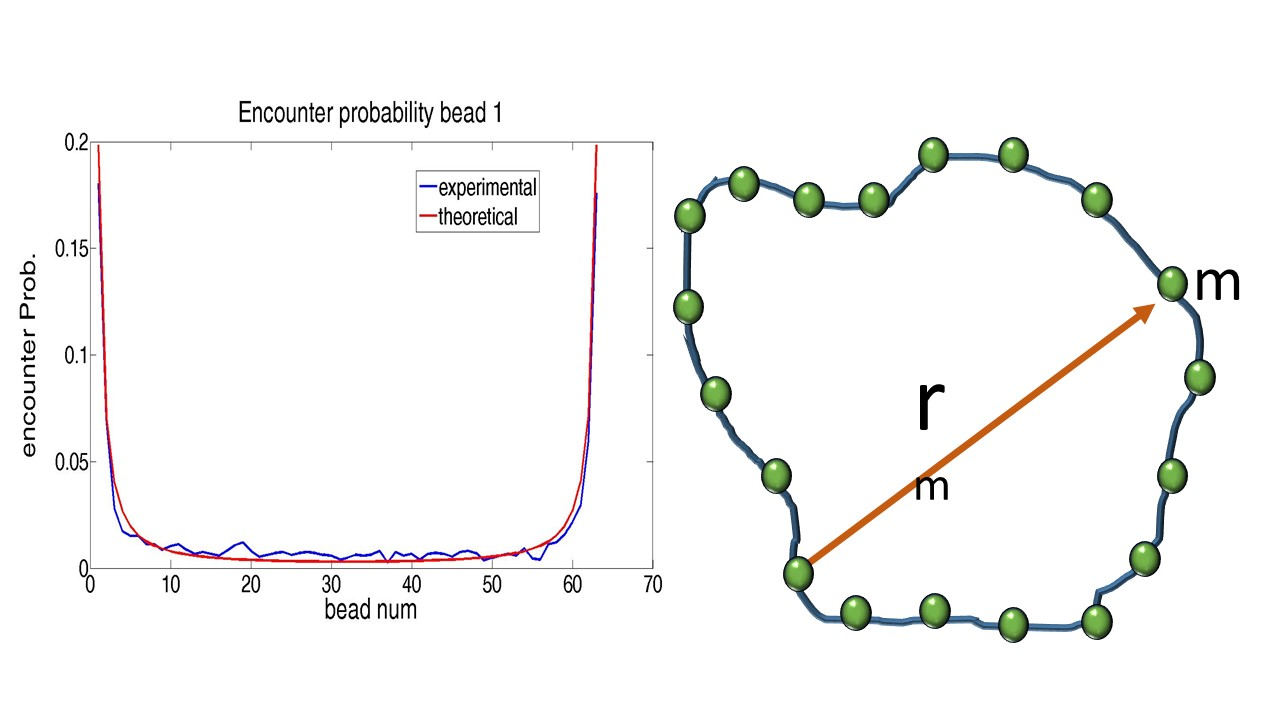
\includegraphics[scale=0.2]{rouseRingVectorBetween0AndM}
\end{figure}
\end{frame}

\begin{frame}{The encoutner probability in composite structures}
The pdf of the vector between bead $n$ of the chain and bead $m$ of the ring is calculated as the sum of the two random vectors $R_{nN_c}$ and $r_m$. 

The calculation can be done using the convolution of the two pdfs, to give
\begin{equation*}
P(r_m+R_{nN_c}=0)=\left(\frac{3}{2\pi b^2(|N_c-n|+m(N_r-m)/N_r)}\right)^{3/2}/S
\end{equation*}
$1\leq n \leq N_c \qquad 0\leq m \leq N_r$ and $S$ the normalization constant 
\begin{figure}
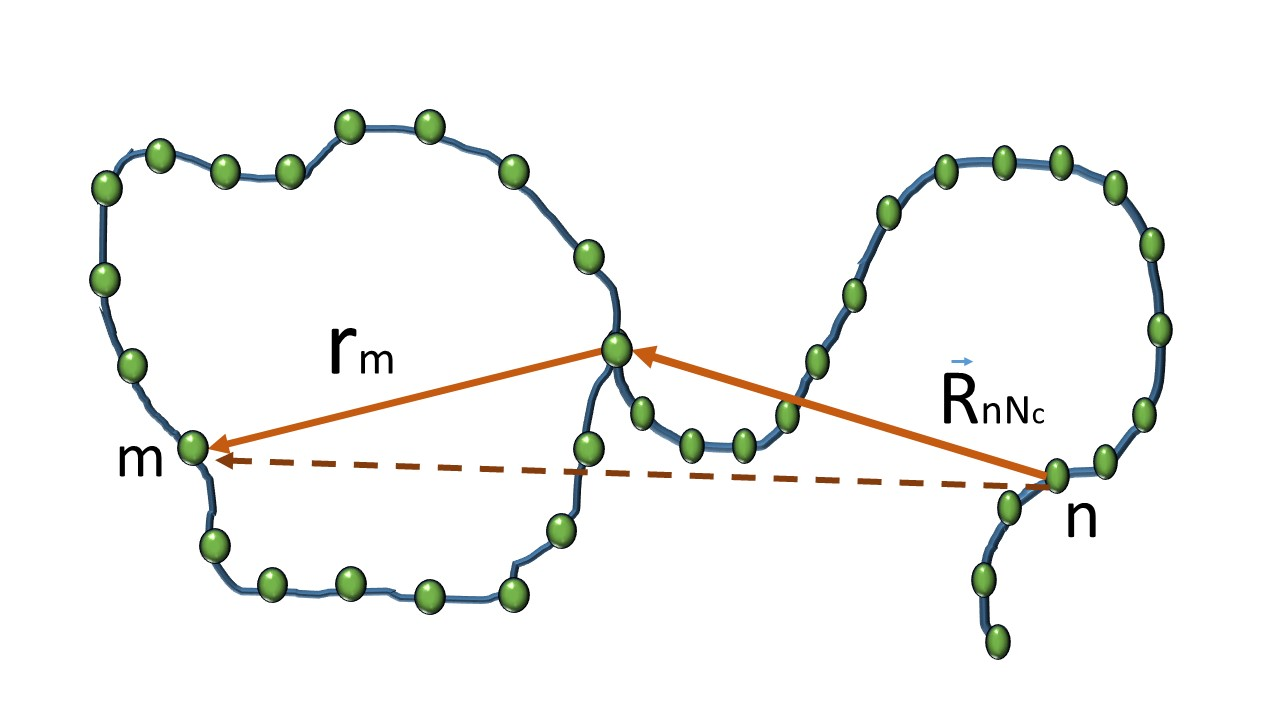
\includegraphics[scale=0.13]{rouseChainAndRingVectorBetweenBeads}
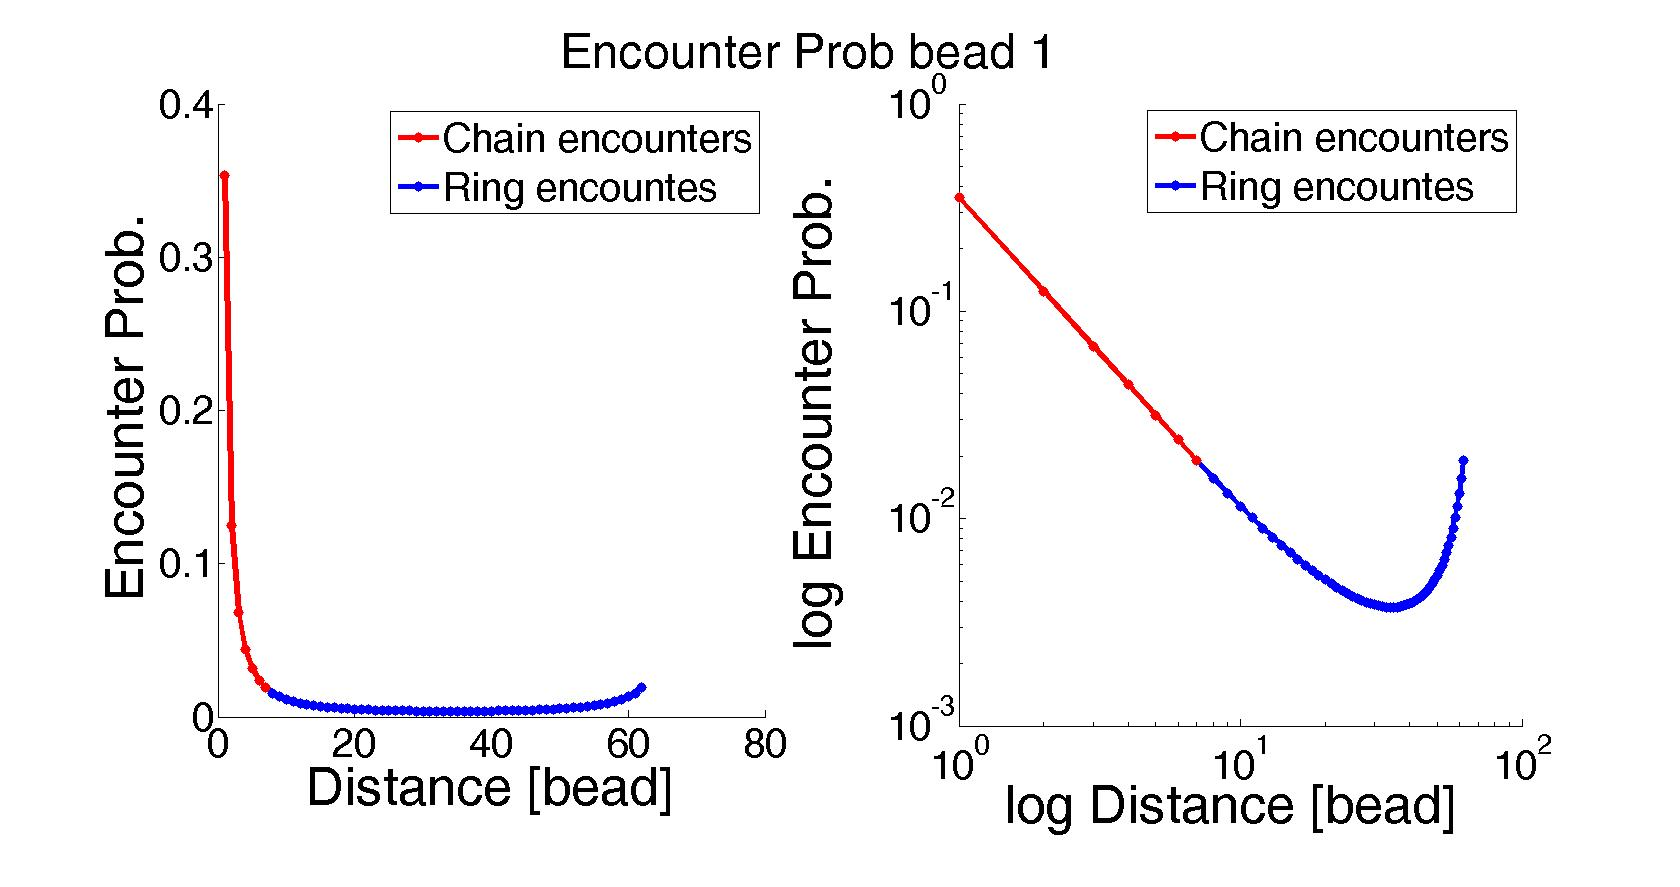
\includegraphics[scale=0.09]{chainRingEncounterTheoreticalProb}
\end{figure}
We can separate the the structures. 
The encounter probability behaves as that of the chain for $1\leq n \leq N_c$ and as a ring for $0\leq m \leq N_r$
\end{frame}

\begin{frame}{From encounter probabilities to distances}
Beads with equal encounter probability are located equidistant along the chain from a reference bead. 
The distance is the shortest one along the graph representing the polymer.

By inverting the encounter probability equation for each structure we can transform probabilities to distances. 

In the case of the Rouse chain 
\begin{equation*}
D_1(P) = \left(P\sum_{t=1}^{N_c-1}|N_c-t|^{-3/2}\right)^{-2/3} \qquad (linear)
\end{equation*}

For the Rouse ring 
\begin{equation*}
D_2(P) =  \frac{N_r+\sqrt{N_r^2-4N_r\left(P\displaystyle\sum_{m=1}^{N_r-1}(m(N_r-m)/N_r)^{-3/2}\right)^{-2/3}}}{2}
\end{equation*}

Using these two structure we'll invert the encounter probability signals from the HiC experiments. 

\end{frame}

\begin{frame}{Interpretation of the encounter signal using chains and rings}
\begin{itemize}
\item we can decompose the HiC signal into regions where the polymer takes a ring or linear chain structure
\item The question is how to find these regions?
\item the positions of the peaks of the signal discloses the model to use.
\begin{figure}[H]
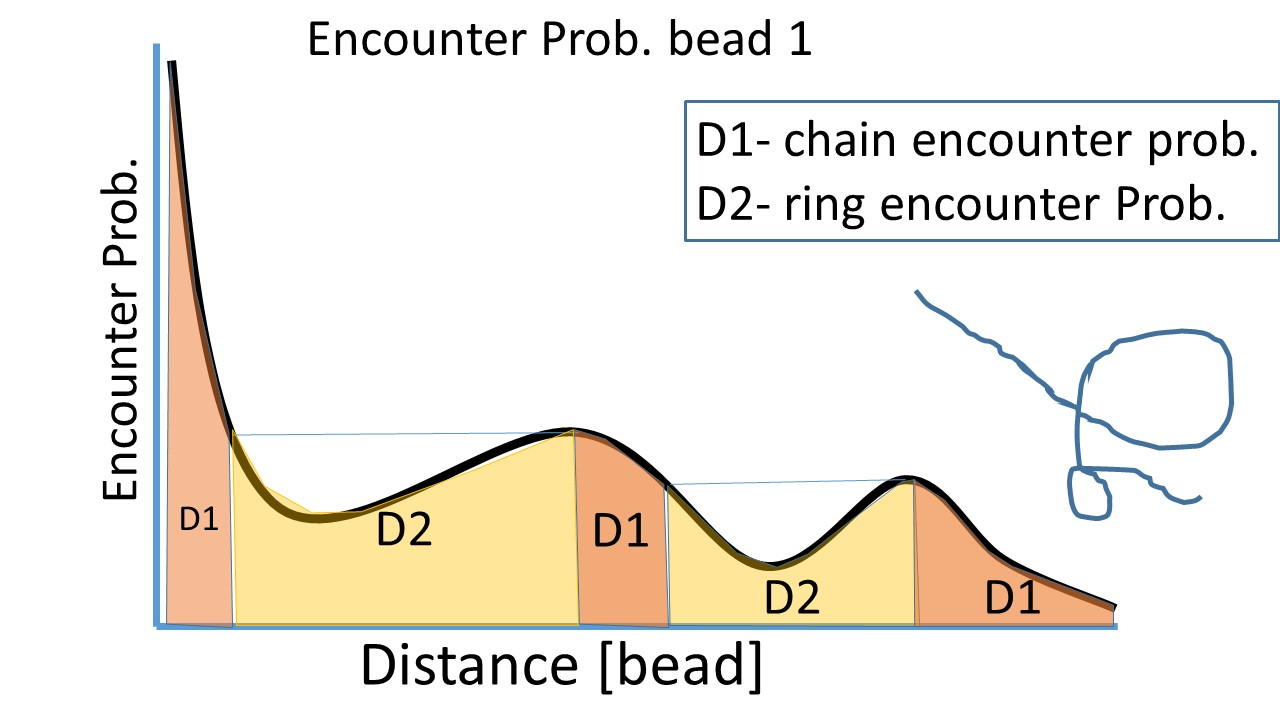
\includegraphics[scale=0.2]{polymerReconstructionTheoreticalApproach}
\end{figure}
\end{itemize}
\end{frame}
\subsection{Validation}
\begin{frame}{Validation}
As an example, we have simulated a  chain of 128 beads with 3 connected loops. Connected bead-pairs: [8 64; 8 120; 38 92; 64 120]. 
\begin{figure}
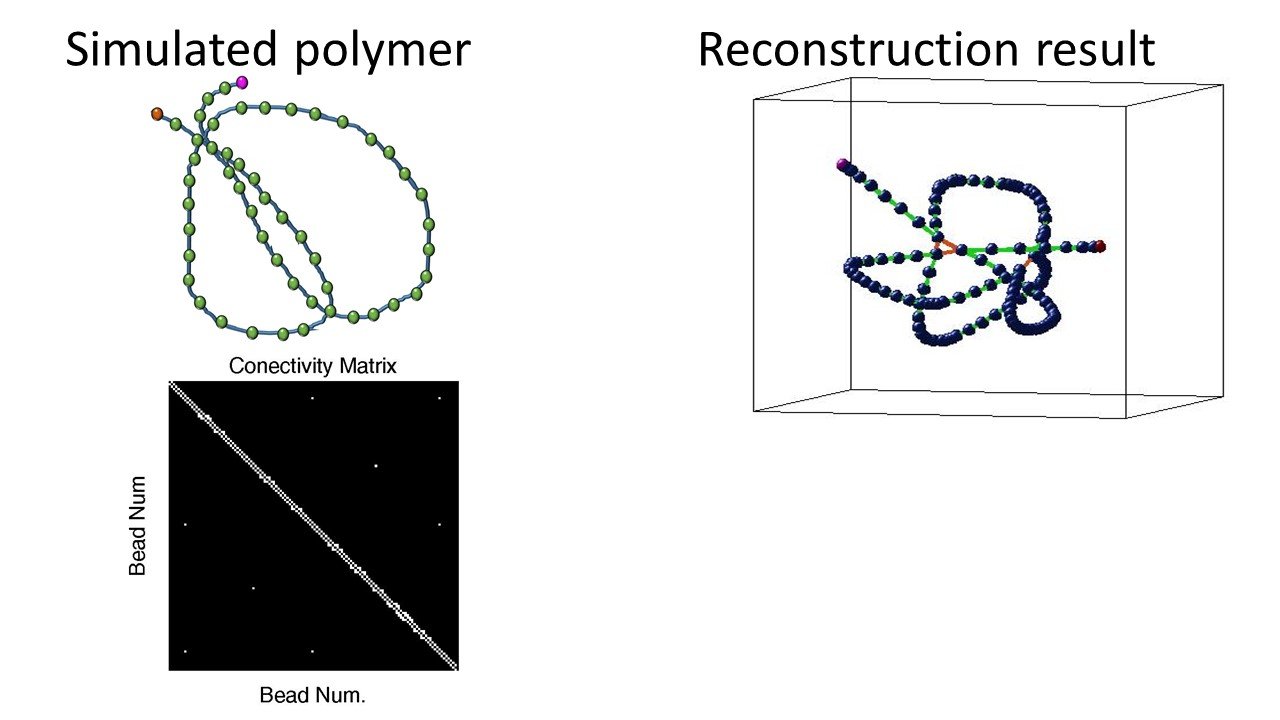
\includegraphics[scale=0.25]{reconstructionResultCompositeStructure}
\end{figure}
The algorithm captures perfectly the prominent features. 

Some off diagonal links were found, which can be eliminated by adjusting smoothing of the encounter signal 

\end{frame}
\subsection{reconstruction of the Experimental data}
\begin{frame}{Reconstruction of TAD D and E}
\begin{itemize}
\item we have tested our method on the experimental data of TAD D and E
\item Prior to the reconstruction we smooth the noisy experimental data
\item For very noisy data we suggest using the curves obtained by fitting $\beta$ values for the transformation of probabilities to distances. 
\item in depth analysis of the resulting structure is underway 
\end{itemize}
\begin{figure}
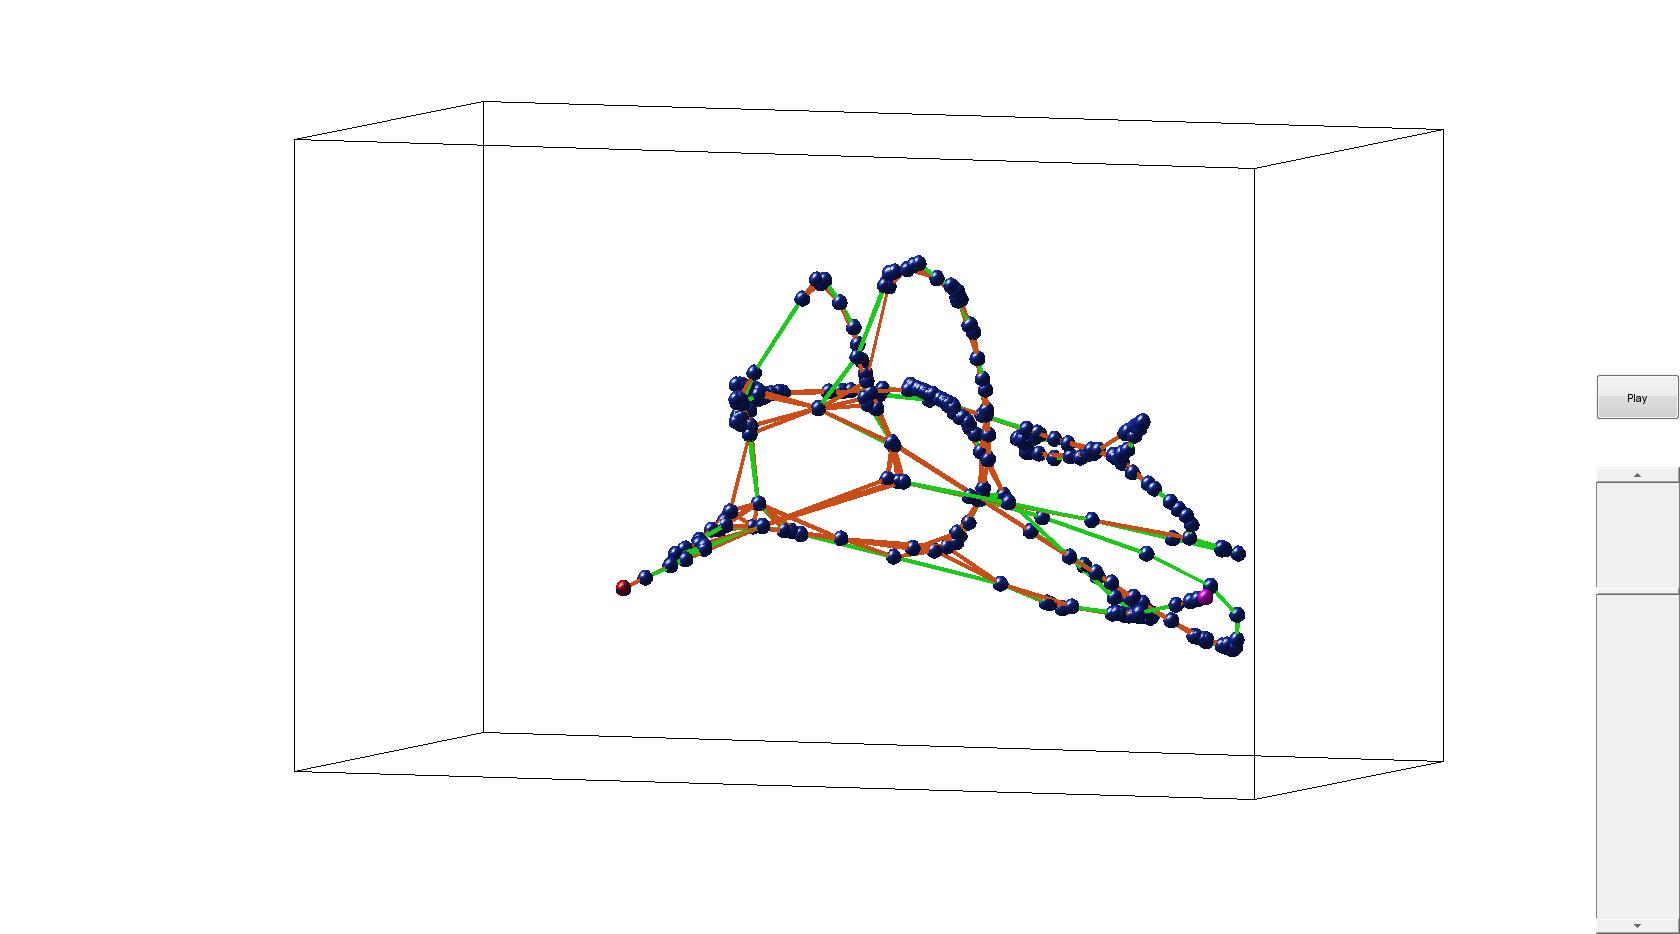
\includegraphics[scale=0.2]{reconstructionTADDAndE}
\end{figure}
\end{frame}


\begin{frame}{Summary}
\begin{enumerate}
\item We have presented a simple method to transform the encounter probability into polymer structure. 
\item The structure is obtained in seconds
\item Prominent features of the structure can be studied 
\item Accuracy is limited by the HiC resolution 
\item simulation to examine conditional encounter probabilities in non-equilibrium states can be performed given the reconstructed structure
\end{enumerate}
\end{frame}

\begin{frame}
Thank you
\end{frame}

\end{document}